%% LyX 2.3.0 created this file.  For more info, see http://www.lyx.org/.
%% Do not edit unless you really know what you are doing.
\documentclass[11pt,english]{article}
\usepackage{tgtermes}
\usepackage[T1]{fontenc}
\usepackage[latin9]{inputenc}
\usepackage{geometry}
\geometry{verbose,tmargin=1cm,bmargin=2cm,lmargin=3.5cm,rmargin=3.5cm,headheight=2cm,headsep=2cm,footskip=1.2cm,columnsep=1.2cm}
\usepackage{array}
\usepackage{float}
\usepackage{amsmath}
\usepackage{amsthm}
\usepackage{graphicx}

\makeatletter

%%%%%%%%%%%%%%%%%%%%%%%%%%%%%% LyX specific LaTeX commands.
%% Because html converters don't know tabularnewline
\providecommand{\tabularnewline}{\\}

%%%%%%%%%%%%%%%%%%%%%%%%%%%%%% User specified LaTeX commands.
\usepackage{mathtools}
\usepackage{amsmath}
\usepackage{xparse}
\usepackage{lscape}
\usepackage[section]{placeins}
\usepackage{bbm}
\usepackage{natbib}
\usepackage{longtable}
\usepackage{booktabs}
\usepackage{sectsty}
\tolerance=1
\emergencystretch=\maxdimen
\hyphenpenalty=10000
\hbadness=10000
\usepackage[left,modulo]{lineno}
\usepackage{soul}
\usepackage{color}

\newcommand{\hly}[1]{{\sethlcolor{yellow}\hl{#1}}}

\makeatother

\usepackage{babel}
\begin{document}

\partfont{\fontsize{12}{15}\selectfont\centering} 
\part*{\centering{Urbanisation Levels and Wealth Effects for Education in sub-Saharan Africa}}
% \subsubsection*{\centering{\textit{A case-study in Tanzania and Nigeria}}}

\vspace{2in}

\begin{abstract}
The economies in sub-Saharan Africa witness high unemployment and
significant wealth effects that limit access to higher education.
The current study compares the importance of wealth effects in Tanzania
and Nigeria for education expenses across varied levels of urbanisation,
access to secondary education and household permanent income in the
two countries. Despite the effects of social and institutional structures
on access to education, the extremity of wealth effects in the poorer
and less-urban economy suggests that a rise in urbanisation may act
to reduce the relevance of wealth for educational attainment in the
region.
\end{abstract}
\onecolumn

%DONE
% 1 (X). No talk about neighbors or reference. There is no plan to discuss the tendencies of keeping up with the neighbours.
% 3(X). Remove all talk about status consumption and of mobility.
% 8(X). Don't talk about deterministic path of needs.
% 10(X). Reference group is also removed - because the measure if that of prosperity (so the concern about normative reference group is to be removed).
% 5(X). Explain why durable goods / assets are preferred over income measures (cite paper). Explain how wealth indexes are prepared.
% 20(X). clarify that it's a cross sectional regression.
% 6(X). Literature on the determinants of education spending, particularly in a developing country context must be discussed.
% 6.1. (X) FilmerPritchettWealthEffectonEduc1999, FilmerPritchettWealthEffectonEduc2001 - compare education attainment in India using SES measures.
% 6.2. (X) ObasuyiEducationInequality2019 - prefer wealth inequality over income inequality. They find significant effects of SES on education access.
% 6.3. (X) WuZhangUnequalEduc2008 - provide a theoretical model for a poverty trap created by education inequality.
% 6.4. ThomasWangEducIneqGini2001 - argue that enrolment measures flows rather than stocks
% 6.5. (X) KambonBusbyEducationPoverty2000 - find effects of wealth on education in the Caribbean.
% 6.6. (N) BehrmanVietnamEduc1999 - .
% 6.7. TanselParentEducEffects1997 - explore the effect of parental education.
% 6.8. ChernichovskySESEnrollment1985 - evaluate whether education is designed for sparsely populated regions or not. They explore in particular if enrolment itsel is influenced (a probit approach). They find that higher number of children increases enrolment.
% 6.9. (N) GlewweJacobyEconGrowthEducDemandWealthEffects2004 - look into how wealth might influence education and see if it's the lower returns to education or the wealth effect that prevents access to education. They are interested in the change in enrolment with economic growth.
% 6.10. (N) GertlerGlewwe1990WTPEduc - find that poor are willing to pay for education in Peru.
% 6.11. NgwareOnsomuKenyaSecEd2006 - find extreme effects of secondary education availability on education.
% 6.12. (X) KakumOlimNairobiSegregation2007 - relate informal sectors with segregation in Nairobi.
% 6.13. (N) SpaullPovertyEducSA2013 - explore effect of poverty / apartheid on education in SA.
% 6.14. EnrolmentDevelopingCountries2009 - PENDING DOWNLOAD.
% 6.15. MaralaniHsizerelEduc2008 - find that for rural cohorts, there is little evidence of a statistically signi cant association between family size and children's schooling. But the re1ationship changes over time. 
% (DONE)9. Discuss equations earlier and write them out.

% 12(X). Don't use individual/consumer/household interchangably.
% (DONE)15. Add what 1. means.
% 16(X). Use urbanisation and justify urbanisation with economic development and wealth. Why not use permanent income cluster instead of long-term durable goods clusters. Instead of urbanisation, are we looking for long-term or wealth that stays over generations? If latter then we need to talk about long-term wealth and that education is rite of passage for the rich. Further, an index based on population may be needed.
% 18(ignored). Also look at breakdown of education costs (books etc.).
% 19(ignored). Look at how school enrolment might have changed in panel data.
% 4. 
% 4.1. Zero expenditure on education, families with no children and household with no assets need to be accounted for  (told how many they are etc.). The fields attended_school is_inschool are fine for TNZ - although current_educ_level  is not much better than highest_educ (in terms of NAs). attended_school is also available for NGR (which can consider withdrawal) while current_educ_level is not. For TNZ: We don't accessibility data for all the wards so we have to simply just take the wards-score. If more wards has accessibile schools then that district is more accessible.
% % 4.2. The heckman solution is based on a binary variable - hence this binary variable must merge the presence of government secondary and government primary schools. One way to merge is to consider primary-school indicator only if current_educ_level points to primary and use second-school indicator if any of the current_educ_level's point to secondary.
% % 2. Discuss how many children are in the household and whether the analysis has a bias due to joint and nuclear families (how many nuclear families etc.).
% % 7. Address that savings on assets is not part of the analysis.
% % 11. In addition of or instead of meanchildage - use dummies indicating age groups of children
% 13(ignored). Use household-income instead of local income differences.
% 14. Don't use symbols for discussion but use the full English name instead.
%  (DONE) 17. Since districts are of varying sizes, district level averages cannot be interpreted as neighborhood effects.

% 20. Glewwe looks at wealth effects using enrolment data over the panel and see whether the wealthier consumers stick to the schools longer.

%%
% (DONE)  24. Literature on urbanisation and education in SSA
% (DONE) 24.1. EbaidallaSudanHHeducExpenditure2018 - use a tobit on household education expenditures to find that households with higher income, residing in urban areas spend more on education in Sudan.
% (DONE) 24.2. DonkohDeterminantsHHEducExpenditure2011 - also find higher urban hh expenditure
% (DONE) 24.3. AcerenzaGandelmanHHEducLatAmCaribb2017 - find that more educated  and  richer  household  heads  spend  more  in  household  education  in both absolute  levels  and as  percentage  of  total  household  consumption in LatAm countries.  This  result  contributes  to perpetuating educational differences over time. Educational  spending  is  highly  unequal. 
% (DONE) 24.4. KnightShiEducRuralUrbanChina1996 - look at urban-rural differences in China. 
% (DONE) 24.1.1. They point out that education is available more widely in the urban than in the rural areas of many developing countries. When education is publicly funded and funding is regionally decentralized, we would expect the extent of educational provi- sion in a region to depend on its income. A prosperous region can afford to devote more resources to education; unless it is cross-subsidized, a poor region can afford less. Given a high urbanrural income disparity, the more rural regions are at an educational disadvantage. 
% (DONE) 24.1.2.1. In market economies, households with more income demand more education as a consumption good. Second, given capital market imperfections richer households can better afford to invest in education. For instance, the foregone earnings cost may bear more heavily on poor households. Third, richer households may have the knowledge, the contacts or the complementary resources which raise the rate of return to education for them. For these reasons we expect household income and the educational attainment of children to be positively related in countries with predominantly private educational systems. Thus, rural-urban income disparities can also generate educational disparities.
% (DONE) 24.1.2.2. In state education economies, the children of educated parents may be at a competitive advantage not only because they tend to inherit greater natural ability but also because they have better opportunities to acquire out-of-school human capital. For instance, they may receive more stimulus from the household environment, absorb more favourable attitudes and have better access to books or to electric light for evening study. In this way educational inequalities can be transmitted from one generation to another.
% (DONE) 25.1. Pitch social influences on education expenditure, urbanisation is related - but the key concern is the social influences in urban areas being different.  The relationship between wealth concentration and education-expenditure is a result of social differences. 
% (DONE) 25.2. The main issues are wealth concentration and urbanisation. 
% (DONE) 26. to research: All the literature on spillover : SOCIAL INFLUENCE ON EDUCATION.
% (DONE) 27. heterogeneity needs to be discussed - probably with a sub-sample - how people are affected is different (heterogeneity) - are they different for poor vs rich  
% (DONE) 28. Compare educational attainment desc-stats for Nigeria and Tanzania.
% (DONE) 29. Literature on determinants of Education and social influence
% (DONE) 29.1. KanellopoulosPsacharopoulosPrivateEducationGreece1997 - find that private education expenditure dominates and wealth effects are significant. They find (Bolivia?) has inelastic education expenditure. They also find that poor spend proportionately higher.
% (DONE) 29.2. TilakDeterminantsHouseholdexpenditureinRuralIndia2002 - also finds that poor spend proportionately higher in India. They argue that one cannot assume the education is free - because the poor do spend high amounts on education (if not on fees then a lot of other related expenses). This is a social cost therefore. Tilak goes on to discuss -  why households invest in education. First, education is not sufficiently free from the govt. Second, they believe that high fees means high efficiency. They're also interested in whether education is  a superior good or not. They find that at an all India level, household expenditures on education are less elastic to changes in household income. They find that Muslims do not spend as much on education. They find that differences by occupational groups in household expenditures on education in government and government-aided private schools are not high; but they are high in private schools. The parental education level does matter significantly in the rural areas. They also use a village-development-index (which is meant to correspond to higher educexp).

% (DONE) 29.3. HashimotoHeathIncomeElasticityEduc1995 - mark differences in elasticity by income
% (DONE) 29.4. AlQudsiFamilyBackground2003 - find the role of parental education in Arab countries.
% (DONE) 29.5. KnightEducationalattainmentRuralUrbanChina1996 - find the evidence of urban-rural divide.
% (DONE) 29.6. QUANGEducationalExpenditureVietnam2012 - use expenditure instead of enrolments.
% (DONE) 29.7. GurlerDemiroglariHHEducDeterminants2020 - also show role of income, parental education, gender and number of children.
% (DONE) 29.8. BayarDeterminantsEducTurkey2016 - Households in urban areas are more likely to make investment for their children since in urban areas it is more likely that education returns are higher.
% (DONE) 29.9. AcarHHEducTurkey2016 - also use the two forms we use i.e. the woking-leser form and the double-logarithmic form. They find significance of parental education, gender and urban-rural effects.
% (DONE) 29.10. GorardEquityComparisonEduc2004 - compare equity in European countries  and find that nationally comprehensive systems of schools tend to produce narrower social differences in intake and outcome.
% (DONE) 29.11. YanPengHHEducChinaSocialClass2021- comment that the segmentation of class educational opportunities has increases with the more opening up/liberalisation.
% (DONE) 29.12. YamamotoCulturalCapitalJapan2010 - explore the role of shadow education (private tutoring etc.) and cultural capital. They find significant effects of teachers judgments favouring high-cultural backgrounds of richer pupils.
% (DONE) 29.13. ByunTheseisCulturalCapitalSouthKorea2007 - find that cultural capital - particularly high-brow participation has negative rather than positive effect on education. This is because the school competitions is time-consuming and pariticpation in high-brow activities takes time away from preparation.
% (DONE) 29.13.1. children from the upper class are more likely than those from the lower class to have cultural capital because they are exposed to cultural dispositions from birth in their families (Bourdieu, 1977, 1997). 
% (DONE) 29.13.2. Those children who have higher cultural capital are likely to do well in school because teachers tend to favor those students with higher cultural capital and thus give them more attention and feedback (De Graaf, De Graaf, & Kraaykamp, 2000; DiMaggio, 1982; Dumais, 2002). 
% (DONE) 29.13.3. DeGraafParentalCulturalCapital2000 - find that it's reading habits rather high-culture-pariticpation that increases school performance. Importantly, they find that a significant part of parental social background could be explained with explicit measures of resources.
% (DONE) 29.13.4. KatsillisGreeceCulturalCapital1990 - find the same as DeGraafParentalCulturalCapital2000.
% (DONE) 28.14. GouldParentalQuality2020- talk about quality (education-level) of parents in the US and how educated parents spend more time with their children.
% (DONE) 30. Literature on urban-rural dichotomy vs spatial distribution
% (DONE) 30.1. WigginsProctorRuralUrban2001 - 
% (DONE) 30.1.1. Take care not to confuse the peri-urban with the rest of the rural. 
% (DONE) 30.1.2. Natural resources might not be the sole criterion to be define rural surroundings. Wealth may evolve regardless of whether their less par-capita land available or not.
% (DONE) 30.2. ChamberlinGeoContextDevelopmentEthiopia2006 - use the population density and access to markets based view of agricultural income. 


% 21. Descriptive Statistics edits
% (DONE) 21.1. Mention if the average number of children are used in Section 6 (Descriptive statistics) 
% (DONE) 21.2. Use percentages for education rank plots (number of households in %)
% (DONE) 21.3. Check order of figures (why 4 after 5)?
% (DONE) 21.4. Write which of occupation rank 1 or 3 is higher?
% (DONE) 22. Describe each column
% 23. Use south-north dummy for Nigeria - to talk about whether higher expenditure on education are aligned southern Nigeria being relatively more industrialised than the northern part of the country.
% (DONE) 31. add a couple of sentences here, picking out some interetsing stats - e.g. the propropriton of households where the head has education level x is x in Tanzania versus x in Nigeria
% 32. 

%[DEMAND Question] - Wealth effects are like gravity for education attainment - but leaving pointing to a general relevance of social factors is not an option. Given that we consider both Nigeria and Tanzania (focusing on NGR alone is an option), the urbanisation - which is a major supply side issue - should be seen highlighted as a measure that compares with the direct measure of educational institutitions are spread in the country. Only thing that is important is the wealth effect - which has two effects - quality of education and social exclusion. We don't have a measure for quality - so we focus only on higher expenditure  on education after controlling for non-durable consumption prices in the region (i.e. if consumer spend more on education with respect to other non-durable expenditure relative to non-durable expenditure). The second issue is to understand if wealth may be limited access to higher levels of education. The lower demand for education could either be due to low returns to education or due to wealth limiting access. As returns to education is not availalbe to us, we are interested only if wealth is preventing access and therefore causes some degree of social exclusion both through wealth (price of education and wealth) and social factors relevant to wealth. 

% A heckman formulation (no schools in the area mean 0 expenditure) could be used to understand the effect of supply-side issues and focus on wealth alone on expenditure.

% Things not done at this point
% 1. Going to primary and then to secondary can also checked with logits and either. 
% 2. The length of schooling time is not available for a huge part of the population so that is excluded.

% To minimise clutter, we can remove the logX and argue that we intend to measure wealth effect alone (rather than logX). The Educ-2012 etc would then disappear. logits could be provided but if we're interested in the expenses, then dummy variables indicating child.in.primary and child.in.secondary might also suffice. We could further minimise by looking at secondary alone. The length of time the students stay in school for (overall) is not available for a large part of the population.

% As such there is little dichotomoy, since the effects are significant for both. One option is to see who has higher wealth effect.  Even for those who are convinced of the dichotomy between the effect of private wealth effect vs urbanisation, more interesting details of segregation (are consumers really being segregated by urban areas needs to be clarified - the measure of urbanisation/wealth concentration/school access drives this. 

%Followup questions:
% 1. Are people not spending on education merely because of access, or does the wealth effect dominate urbanisation.
% 2. What about children being mixed with adults?

% \section*{\centering{Research Question}}

\noindent
% In the context of developing economies in sub-Saharan Africa, is the spending on education more often determined by the concentration of wealth in the household's area of residence than by the permanent income of the household?

%1. We already talked about the endogeneity and it does not matter - since we're interested in relative effect of A and r.
%2. Wealth people live in wealthy neighbourhoods but I am not looking at neighborhoods - urbanisation is observed at a higher level than neighborhood.

\section{\label{sec:Introduction}Introduction}

% One possible highlight is that wealth effects need not be significant in a cross country comparison - both the secondary school availability and urbanisation are important. The importance of secondary-schools and urbanisation may need to be sold more directly in the introduction because the results are effectively downplaying the role of wealth effects. 
% [INTRO-LINE] Wealth effects are highlighted a lot. We use urbanisation measures against physical access to find that education expenditure rises more significantly with the rise of urbanisation - which is measured using an improved sense of wealth concentration.

\noindent

%[Wealth effect weaken policy and we look at wealth effects]

The participation rates for secondary and higher education remain
one of the lowest for the economies of sub-Saharan Africa (SSA). Education
remains inaccessible to the vast majority and inadequate in providing
mobility to those with low-income who do acquire it (\cite{dabalenNigeriaUnemployment2001,oketchAfricaHE2016,NdyaliHE_Unemployment_TNZ2016,MinnisNonformalEducation2006}).
The low participation in education has been attributed both to an
insufficient focus on non-formal education (\cite{MinnisNonformalEducation2006}
) and the barriers imposed by inadequate wealth (\cite{GlewweJacobyEconGrowthEducDemandWealthEffects2004,IliePaulineWhobenefitsfromHE2018}).
In the presented chapter, we examine whether the changes brought about
by urbanisation in SSA may act to reduce or worsen the effect of long-term
wealth (i.e. wealth effects) on education expenditures. Comparing
the role of urbanisation across Tanzania and Nigeria - economies which
we select due to significant differences in levels of urbanisation
and degree of dependence on agrarian production - we find that the
significance of household wealth on education declines with higher
urbanisation in the region.

The wealth effects on education - i.e. the extent to which the household
wealth contributes to education expenses - are commonly observed through
various mechanisms (\cite{GlewweJacobyEconGrowthEducDemandWealthEffects2004,IliePaulineWhobenefitsfromHE2018}).
Other than through costs (such as transportation) imposed on households
when public education access is poorer, household wealth also influences
access to education due to information symmetries that may help in
future job-searches, better representations in the nascent political
institutions of developing economies or certain social characteristics
that align with higher local (relative) household wealth (\cite{BehrmanVietnamEduc1999}).
As higher intergenerational wealth may help fund higher levels of
education, the wealth inequalities tend to become educational inequalities
by creating a poverty trap for the lower-income households (\cite{GlewweJacobyEconGrowthEducDemandWealthEffects2004,BehrmanVietnamEduc1999}).
This has been an important concern for policy in SSA due to the predominance
of large informal sector in the region and the higher consequent income
volatility that could deprioritise education expenditures for poorer
households (\cite{KakumOlimNairobiSegregation2007,OwusuGhanaSegregation2011,MinnisNonformalEducation2006}).
Such effects evidently get worse at higher levels of education as
the foregone labour income through time spent in education becomes
costlier for households with low possessions or wealth. The empirical
literature often suggests a stronger role of wealth effects than physical
access for education expenses in the literature (\cite{GlewweJacobyEconGrowthEducDemandWealthEffects2004,BehrmanVietnamEduc1999}).

% [measuring wealth and urbanisation]

While we measure wealth effects as the annual total household expenditure,
the effects of urbanisation - whose effects we wish to detail in the
current chapter - are interpreted as that of wealth-concentration
in the immediate area surrounding the household. The goal of the particular
notion of urbanisation as a measure of concentration of wealth is
to take into consideration the spatial variation in the SSA while
standardising the measurement of urbanisation across different economies.
More specifically, the measure of urbanisation as concentration of
wealth relies on the market value of assets\footnote{The term ``assets'' signifies the goods that are owned by the household.
These constitute items that are more often referred to as durable
goods in the consumption literature from the developed economies.
There seem at least two reasons why the developing economics literature
more often refers to the durable household possessions as assets.
First, the financial assets are far less relevant in the developing
economies. Second, the durable goods such as bicycles or stoves -
however insignificant - are far more important for consumption behaviour
in the developing world.} owned by the household that are recorded in the consumption survey.
While several empirical studies use urban-rural effects to explain
disparities in education expenditures in SSA (\cite{EbaidallaSudanHHeducExpenditure2018,DonkohDeterminantsHHEducExpenditure2011})
as well as in other developing economies (\cite{BayarDeterminantsEducTurkey2016,KnightEducationalattainmentRuralUrbanChina1996,AcarHHEducTurkey2016}),
recent studies highlight the need to consider spatial distribution
of resources and employment opportunities in the SSA - instead of
the broad or implicit urban-rural classifications that are often used
in surveys (\cite{AbayYoungRuralEconomy2021,WigginsProctorRuralUrban2001}).
These concerns are what motivate the use of wealth-concentration as
the primary measure of urbanisation in the current study.

%[Effect of urbanisation ]

The urban-rural disparities influence participation in education through
various mechanisms. Setting aside the physical access to education
- the higher availability of education opportunities in urban areas
which we consider as a separate control - the fundamental mechanisms
we intend to focus on through a measure of urbanisation are the relative
abundance of opportunities for higher income employment and the social
environment of the urban areas. The better opportunities of employment
and wealth overall make education more affordable so that the rural
households - where incomes are invariably lower and education somewhat
of a luxury- end up underinvesting in education. The social environment
of urban areas is often different - leading to a stronger need for
finding education-dependent employment in urban areas. Both of the
factors constitute the positive externalities from being in a rich
locality (district) that are encompassed in the measure of urbanisation
- a measure driven by the concentration of richness in terms of assets.
More specifically, the study measures urbanisation with the average
assets values in the household vicinity - while explicitly accounting
for other social factors pertaining to the household (religious identity
etc.) and controlling for availabililty of education opportunities.

The wealth concentration interpretation of urbanisation also assists
us in empirically distinguishing the effects of urbanisation from
household wealth effects. This is foremost because the asset values
used in the wealth concentration and the total budget expenditure
used in the permanent income (\cite{modiglianiutility1954,FriedmanConsumption1957})
are measured independently in the survey - avoiding the need to rely
on any community-level fields (characteristics of village, ward etc.
assigned in the survey) for assessment of urbanisation-levels.  To
compare this assessment with a more conventional approach using urban-rural
indicators, we also provide estimation results with an alternative
formulation where a ruralness-score of the district based on urban-rural
distinction in the survey is used as a measure of urbanisation and
household-wealth is measured using the assets owned. The primary wealth-concentration
interpretation of urbanisation - which interprets urbanisation as
concentration of long-term asset ownership in a 6-$km$ area \footnote{This 6-$km$ scale in the district where the household residence is
located - is based on the geographical distances between districts
and the average distance to the education facility recorded in the
consumption survey.} - provides a continuous (rather than categorical) variable for urbanisation
levels. The wealth effects - measured as effects of household wealth
on its education expenditures (\cite{GlewweJacobyEconGrowthEducDemandWealthEffects2004})
- are then contrasted against the urbanisation effects (which include
the positive externality from being in a wealthy area). With wealth
effects and urbanisation effects thus compared after controlling for
physical access and social factors, we find that the wealth effects
for education to be more severe in less urbanised areas.

%[physical access - an important control] - We don't use secondary + primary because an aggregation to district - which is needed - cannot be justified. 

The physical access to education - a factor that directly influences
education expenditure - is an important control in the above analysis.
Given the focus on secondary education in development policy as well
as literature in the last decades (\cite{FullerVocationalTraining1976,TilakEducationPoverty2002,TilakPostelemEducIndia2007,HeynemanHistoryProblemsWorldBank2003,heynemanInvestmentIndianEducUneconomic1980}),
we focus on the accessibility of secondary education in the two economies.
Controlling for physical access is relevant also because poor education
access might make wealth effects appear stronger (due to higher transportation
costs etc.). The control in fact often plays a critical role in determining
whether a given amount of funds is more appropriately used to build
accessible schools or to support and economise education instead.
More specifically, if physical access for education is what prevents
the attainment of education, then building more schools becomes of
higher priority. On the other hand, if wealth effects are stronger
in the economy, then affordability of education becomes an important
issue - even if returns to education were a cause of concern. Whether
returns to education are enough to increase education participation
for lower-income households or not also often hinges on there being
less significant wealth effects and sufficient physical access to
education in an economy (\cite{GlewweJacobyEconGrowthEducDemandWealthEffects2004}
). The results we obtain with urbanisation levels are particularly
significant since the wealth effects are more often reported to be
stronger than the effects of physical access in empirical studies
from the region (\cite{ObasuyiEducationInequality2019,FilmerPritchettWealthEffectonEduc1999,FilmerPritchettWealthEffectonEduc2001,MinnisNonformalEducation2006,BehrmanVietnamEduc1999,GlewweJacobyEconGrowthEducDemandWealthEffects2004,KambonBusbyEducationPoverty2000}).

%[Urbanisation and social effects]

The social environment of a household is another important control
that one cannot ignore as the factors influencing participation in
education. While the effects of discernible factors such as segregation
or exclusion based on social identities education have been often
highlighted in SSA (\cite{KakumOlimNairobiSegregation2007,OwusuGhanaSegregation2011}),
the specific role of social factors that may encourage or support
education present a more challenging task to the empirical studies.
Early attempts to explain the role of social factors have advanced
the notion of social capital (\cite{BourdieuCulturalRepr2018}) -
which encompasses habits, preferences and behaviour cultivated in
richer environments that affect future educational mobility. The empirical
studies pertaining to social capital - however emphasise more often
on certain environmental factors - such as the feedback for improvement
of students, the subjective evaluations of students or other measures
of social interactions (\cite{Manski2000})- rather than any claimed
role of a ``higher-culture'' (\cite{YanPengHHEducChinaSocialClass2021,YamamotoCulturalCapitalJapan2010,ByunTheseisCulturalCapitalSouthKorea2007})
that may influence participation or success in education. As empirical
measures for social capital have neither been considered universal
nor equivalent to physical in the empirical literature(\cite{SobelSocialCapital2002}),
we prefer to focus on specific social factors at the household level
in the current study.

% The use of occupation as a control also allows us to test if it is more often that the non-agrarian workers treat education as a basic need for the occupations they aim for (all else being the same) or if it is the agrarian sections instead who spend more on education (when accessible) - viewing it as the only way out of poverty ([#TilakDeterminantsHouseholdexpenditureinRuralIndia2002]). 

These social factors encompass the acquisition of skills from parents
or from the social environment (networks) valued in the employment
markets and higher levels of education. The parental educational levels
- which are widely observed to have a significant effect on education
attainment in the developing economies (\cite{TanselParentEducEffects1997})
- are the first important social factor. It is also possible to argue
- from a certain human capital perspective (\cite{WuZhangUnequalEduc2008,BehrmanVietnamEduc1999,GlewweJacobyEconGrowthEducDemandWealthEffects2004,SpaullPovertyEducSA2013})-
that the effect of parental education levels is not unlike the effect
of wealth (which has a strong effect on educational expenditures)
since both accumulations are transferred to further generations (\cite{BeckerTomesEquilibMobility1979}).
The other important factor considered in the current study that may
favour participation in education is the main occupation in the household.
More particularly, the agrarian or non-agrarian nature of the household
occupation in a largely agrarian economy may indicate a non-transactional
advantage for individuals through the social networks they acquire.
Other household characteristics of social significance that influence
participation in education vary across the economies. In Tanzania,
for example, the speakers of English language seem to be generally
more educated and have higher incomes. The ability to speak English
could indicate an exposure to education in ways that the poorer or
rural households may not be exposed. The religious identities also
have some implications for participation in education in countries
such as Nigeria (\cite{CorrayPotrafkeGenderPolitics2011,AlesinaMobilityAfrica2019}
). 

%[Household-size]

An essential claim of the human capital theory (\cite{TilakEducationPoverty2002})
- which the empirical literature on determinants of education expenditure
often relies on - is that the educational investments must change
over the life cycle of consumers. The current chapter takes advantage
of the reporting of household expenditures on education at individual
level in the surveys for both the countries and considers how the
education expenditure may vary with the age of the children in the
household. The variables for childrens' ages are important for our
comparison also because the education expenditures for a population
where the majority joins the workforce after attaining primary education
would be very different from one where the employment opportunities
are higher for educated individuals. Since large households have higher
basic needs than smaller households, we also consider the number of
children as another relevant control that is closely related with
lifecycle concerns. It is worth highlighting that while one may expect
the household expenses on education to decline with the rise in number
children due to a higher cost pressures, studies often find that education
enrollments to rise instead of decline with the number of children
in some sub-Saharan African countries (\cite{ChernichovskySESEnrollment1985,MaralaniHsizerelEduc2008}
)\footnote{A caveat in such observations is the use of enrollment data - which
has criticised in favour of educational expenditure on the basis for
former measuring ``flows'' rather than ``stocks'' relevant to
education (\cite{ThomasWangEducIneqGini2001,ObasuyiEducationInequality2019}
).}.

%[importance of wealth concentration ]

Considering the role of social factors, it is worth emphasising how
a particular sense of urbanisation also helps us separate the effects
of wealth concentration from the social factors identified above.
The measure of wealth-concentration as inter-generational long-term
assets quantifies urban-rural disparities and allows us to assess
the extent to which a higher wealth concentration may provide a more
supportive environment for education participation after accounting
for the effects of wealth, occupation in the household, the physical
access in the region (the district boundary in the surrounding 6-$km$
distance) and other factors of social significance. The particular
interpretation of urbanisation is based on suggestions to consider
spatial distribution of assets in the recent literature - which has
emphasised the network of occupations and contractual relationships
surrounding the ownership of land or natural resources in SSA (\cite{KoseGhebruLandEthiopia2018,Chamberlin2020ZambiaRuralinmigration,ReardonHHIncomeDiversificationLandOwnership1997})
and highlighted inadequacies of the conventional urban-rural dichotomy
based on categorical variables from community surveys that may not
consider the spatial distribution of wealth and markets in SSA (\cite{AbayYoungRuralEconomy2021,WigginsProctorRuralUrban2001}).

%[Preview results - wealth effects dominate in one over the other and wealth concentration overall important]

As mentioned earlier, the two economies in SSA that we have selected
for our comparison of education expenditure have different levels
of economic development and a different degree of dependence on agrarian
output. More particularly, Nigeria relies more heavily on energy exports
while Tanzania's economy is more reliant on its agricultural output
- a difference that is critical for the varied level of urbanisation
in the two economies. While the educational attainments in the populations
of the two countries are evidently shaped by the idiosyncrasies of
the policy and distinct social factors, the varying levels of urbanisation
in the two economies allow us to explore the challenges that improvement
of employment opportunities and economic development may bring towards
access to education in the region. More particularly, if wealth effects
matter less in the urbanised areas i.e. if education is more egalitarian
for residents in the urban areas (after controlling for physical access),
then the policy may not need to focus on wealth effects and direct
the attention to improving access elsewhere instead. On other hand,
if wealth effects are significant despite higher economic development
in urbanised regions, then more attention is needed for improvement
of access to education for lower-income households.

%[Measurements] - Variables : {wealth,wealth-conc/ruralwards,secondary_schools,occupation, parental education, language-religion, age, numchild, educpriv}

To summarise, household wealth and urbanisation levels are the main
explanatory variables in our comparison of educational expenditures
while physical access to education, the social or demographic factors
and the household characteristics serve as important controls\footnote{Since urban households evidently have higher wealth, a comparison
of urbanisation and wealth effects is not without concerns of a correlation
between household wealth and urbanisation. However, as the study is
concerned only with the relative importance of urbanisation and permanent
income measures in the two countries - rather than the elasticities
of expenditure, these issues are less relevant to the comparison of
household educational expenditure.}. The first explanatory variable i.e. the wealth or the permanent
income of the household uses the logarithm of household's total annual
expenditure. The use of total expenditure as permanent income is common
in studies on consumption and relies on standard consumption theory
(\cite{modiglianiutility1954,FriedmanConsumption1957} ). The urbanisation
levels correspond to a wealth-concentration measure that is used as
the second explanatory variable (see Section \ref{subsec:Results}
for details). As mentioned earlier, the wealth-concentration measure
is simply the average asset-ownership levels in the households' vicinity.
Notice that apart from taking spatial considerations across wider
geographical scales into account, the wealth concentration measure
also avoids the population density based approaches due to issues
arising of densely populated rural areas in SSA economies (\cite{hendersonurbanizationSAADifferent2013,Chamberlin2020ZambiaRuralinmigration,AbayYoungRuralEconomy2021}).
The physical access to education - is measured with the number of
secondary schools in every district so that a higher score of ``secondary\_schools''
for a district implies more secondary schools in the district. Further
robustness checks are conducted by redefining the wealth concentration
measures which vary the boundaries of households vicinity and examine
the significance of wealth-concentration in the household's neighborhood
of similar occupations (agrarian/non-agrarian) and education ranks
(primary,secondary).

In the alternative formulation - which we provide for a comparison
with a more conventional approach using urban-rural demarcations from
the survey - the total value of long-term assets owned by the household
i.e. the measure of household wealth is used as the first explanatory
variable and a ``ruralness'' score based on urban-rural indicators
from the survey is used as the second explanatory variable. The use
of wealth-indices based on the stock of durable goods (excluding short-term
durable goods that are not transferred over a generation) is also
common in the studies from health and household economics (\cite{HoweHargreavesWealthIndices2008,HoweHargreavesWealthIndexComparison2010,McKenzie2005,BooysenVanderbergAssetIndex2008})\footnote{Instead of using income-data, the empirical studies for education
more often rely on the data on ownership of assets (\cite{FilmerPritchettWealthEffectonEduc1999,FilmerPritchettWealthEffectonEduc2001})
- since the inter-generational transfers of wealth are what make a
break in the inequality gap (i.e. mobility through reduction of wealth
differences) difficult (\cite{ObasuyiEducationInequality2019}). }.

% REMEMBER to REMDIND AUDIENCE: Note also that the issues of intra-household allocation of educational expense among children are not relevant to our cross-section analysis since as they average out over multitude of households.

%[Macro literature and conclusions for migration]

The main finding from the current study is that a higher urbanisation
is correlated with lower severity of wealth effects in the region
considering the two economies. While the higher urbanisation may itself
depend on the country's governmental efficiency, natural resources
or fiscal condition, it does seem to reduce the wealth effects on
education. Despite the peculiarities of inequality in SSA such as
high land-labour ratios and sparse distribution of economic resources
(\cite{AndersoninequalityandvariableSAA2004}), therefore, the weakening
of wealth effects with rising urbanisation points in a promising direction
- through rise in employment opportunities - and marks past success
in education improvements in the region. The study also finds that
the segregation of education opportunities and the disparities in
future employment opportunities across the country are more evident
in Tanzania where the differences between urban and rural prosperity
seem more extreme. The other side of the seemingly desirable effects
of urbanisation, therefore, is that the need to improve to education
participation in less urbanised areas remains a significant challenge
for policy. The recommendations for addressing non-formal education
and improving basic education for rural populations may therefore
be an important concern for an education policy when urbanisation
is not readily achievable for the economy.

%[Contributions]

The current chapter contributes to the literature on determinants
of education in two different ways. First, it demonstrates that despite
the challenges of urban overpopulation, the effect of urbanisation
may be a desirable one for the education levels of the population
and the lifestyle improvements in urban areas. This may support the
conventional view that despite the evident problems with rise in inequality,
the urbanisation may play a key role in economic growth through rise
in employment opportunities and income from higher paid occupations
(\cite{KuznetsEconomicGrowthIneq2019} ). More particularly, the weakening
in severity of wealth effects with the rise in urbanisation could
indicate the pathways to future improvements in income equality and
reduction in education inequalities through developments of the industrial
sector and rise in demand for education. The second contribution of
the chapter is the delineation of links between levels of economic
activity and education levels - which we perform considering the spatial
concentration of wealth and education across the two economies. While
most of the literature we have surveyed has focused on the urban-rural
dichotomy from community, the current study relies on the spatial
distribution of wealth to examine the specific link between wealth-concentration,
occupational levels and education expenses in the region.

In the sections that follow, the Section \ref{sec:Literature-Survey}
surveys the literature on education expenditures, Section \ref{sec:Econometric-Method}
details the method used in empirical analysis, Section \ref{sec:Data}
describes the data used for Nigeria and Tanzania in the study and
Sections \ref{sec:AnalysisAndResults}, \ref{sec:Conclusions} discuss
the results from the empirical analyses.

\newpage{}

\section{\label{sec:Literature-Survey}Literature Survey}

\noindent

\let\oldquote\quote \let\endoldquote\endquote
\RenewDocumentEnvironment{quote}{om}   {\oldquote}   {\par\nobreak\smallskip    \hfill{#1}\endoldquote     \addvspace{\bigskipamount}}
\begin{quote}[\textit{Beyond contentment}, John Kenneth Galbraith, (1994)]{} There is no well educated literate population that is poor, [and] there is no illiterate population that is other than poor.  \end{quote}

%[Education Needs]

While education may not be considered a basic necessity in all poverty-measurement
surveys, it is seldom disputed that a lack of education contributes
to poverty. Even in the developing economies, the poorest individuals
might have a strong demand for education (\cite{TilakEducationPoverty2002,GertlerGlewwe1990WTPEduc}).
The literature also suggests that when education is not state-funded
in the developing economies, there might be a compulsion - rather
than a mere willingness - to pay for education among the poor (\cite{TilakEducationPoverty2002,TilakDeterminantsHouseholdexpenditureinRuralIndia2002}).
With a high demand for educated workforce in an industrialising economy,
there seems little disagreement in policy therefore - whether from
a human capital perspective (\cite{BarroEconomicGrowthEduc,BarroHumanCapitalGrowth1999})
or the capability perspective (\cite{SenInequalityReexamined1992,SenNotesonPoverty1978,NussbaumCapabilities2003})
- that economic growth bears a strong relationship with educational
attainment.

%[WE exists]

An important consideration for education attainment in the population
is that while higher education does provide skills for higher incomes,
the expenditure on education tends to be often limited by the wealth
one possesses. The differences in education elasticities based on
income have in fact been emphasised in the literature early on since
the mid-last century (\cite{BensonEconomicsofPublicEduc1961,HashimotoHeathIncomeElasticityEduc1995}).
The empirical studies from the SSA also report significant wealth
effects on education (\cite{GlewweJacobyEconGrowthEducDemandWealthEffects2004})
. Inspecting the enrollments data, for example, \cite{ChernichovskySESEnrollment1985}
note that the children from households that have large cattle stocks
face less reductions in enrollment, because higher wealth may allow
the households to take care of the cattle and prevent the childrens'
withdrawals from schools\footnote{One caveat with the use of education enrollment data is that they
are often not considered rigorous for empirical assessments - as they
ignore the difference in educational levels and measure ``flow''
rather than ``stock'' with respect to educational inequalities (\cite{ObasuyiEducationInequality2019,ThomasWangEducIneqGini2001}).}. Using a benefit incidence analysis to test if the education is pro-rich,
\cite{IliePaulineWhobenefitsfromHE2018} show that the poor young
people receive only 5\% of funds allocated to tertiary education compared
with 54\% for the rich. 

While the wealth-effects remain significant in SSA, much of the discussion
on the high graduate unemployment and low higher-education participation
has focused on the poor returns to education in the region. On one
hand, the literature attributes these problems to the prevalent mismanagement
in public education (\cite{languilleeducbudgetpolitics2019}) and
on the other it highlights a misplaced focus on formal education in
the informal economy settings (\cite{MinnisNonformalEducation2006}).
Instead of focusing on the returns-to-education, we argue that the
poor returns may not offer a complete view of lower participation
in education. One reason is that the education needs or perceived
value of education may not be adequately captured with a returns-to-education
approach. As \cite{HeynemanHistoryProblemsWorldBank2003} point out,
the returns-to-education approaches tend to ignore the positive externalities
from education\footnote{In a debate on whether the policy should favour free basic education
to all (at the point of use) over the investments in higher education
or not, \cite{HeynemanHistoryProblemsWorldBank2003,heynemanLDCOECDSchoolAchievements1980}
argue that the positive externalities from education are simply not
factored in the productivity measures used in the returns-to-education
approach proposed by \cite{PsacharopoulosReturnsToEducation2004}.
\cite{heynemanInvestmentIndianEducUneconomic1980} elaborate that
the individuals benefit culturally and physically from education and
that such changes are ignored when using a returns-of-education approach.
It would seem also that not only does formal education help workers
pick up more skills on their own (\cite{FullerVocationalTraining1976}),
the skills from secondary or higher education are often necessary
in the labour market (\cite{TilakPostelemEducIndia2007}).}. The other reason is simply that the role of physical and wealth
may be far more dominant than the issue of poor returns-to-education
in an economy.

The positive externalities from education - which one may use to argue
that the returns-to-education perspective is an incomplete one - are
less of an issue in the context of SSA. Many empirical studies in
fact report several instances of waste in rent-seeking activities
after graduation in the SSA (\cite{oketchAfricaHE2016,MinnisNonformalEducation2006,dabalenNigeriaUnemployment2001}).
The case for positive externalities from education is weakened further
due to the low economic growth experienced by the countries in the
last decades - a slide that may have suppressed the value of secondary
or higher education in the region. Even though the concerns for return-to-education
remain important, they need to be viewed in the context of wealth
effects and availability of education facilities. More specifically,
it is possible that the demand for education is suppressed due to
inadequate income (relatively high prices of education) in the economy
or a sparse distribution of education opportunities rather than due
to lower pay from post-education employment opportunities alone (\cite{GlewweJacobyEconGrowthEducDemandWealthEffects2004}
). Therefore, if education expenditures are better explained with
physical access, then the policy may need to focus on building more
accessible schools whereas if wealth-effects are more significant,
then there is a need to make education more affordable for the lower-income
households. 

In the context of SSA, the empirical studies have generally found
that the physical access is less significant than the wealth effects
(\cite{FilmerPritchettWealthEffectonEduc1999,KambonBusbyEducationPoverty2000,ObasuyiEducationInequality2019}
). There is some evidence that the effects of physical access do become
stronger at higher (secondary and tertiary) levels of education (\cite{NgwareOnsomuKenyaSecEd2006}).
The effect of urban-rural differences - which may be correlated with
difference in both physical access and wealth concentration - has
also been widely reported to be significant in SSA (\cite{IliePaulineWhobenefitsfromHE2018,castrolealPoorBenefitAfricaEducation1999,GlewweJacobyEconGrowthEducDemandWealthEffects2004,BossuroyCogneauMobilityAfrica2013}).
Both urbanisation-levels and wealth (aside from the physical access
to education used as a control) - are thus important concerns in the
current study that motivate our exploration of the decline in wealth
effects with rise of urbanisation.

% Some studies have gone as far to suggest that education serves as a rite of passage for the urban rich in the economies ([#oketchAfricaHE2016, #MinnisNonformalEducation2006]). 

Another way to interpret the effect of a standardised wealth-concentration-based
measure of urban-rural differences is to contrast local vs wider wealth
disparities that prevent access to education. In other words, the
wealth-concentration interpretation of urbanisation helps us explore
whether the effects of a wealthier locality have a stronger influence
on education than household income or not. As \cite{porzio2021human}
report, for example, the changes in social environment of the urbanised
areas may create a more competitive setting over time and across the
wider populations.The specific wealth-concentration sense permits
a clearer view of the role of social factors as well - since the urban-rural
labels of the survey could encapsulate social divisions - such as
ethnic or socio-economic differentiations in the society being surveyed. 

%[Social Capital is tricky]

The effects of social factors on education - particularly the link
between cultural capital and education - has been of interest in the
sociological literature since the beginning of the post-war era (\cite{BourdieuCulturalRepr2018}).
While this early research had viewed education as a certain high-culture
participation that enhances the social capital of a household, the
later refinements have focused on the specific role of social networks
and parental acquisitions or skills (\cite{ByunTheseisCulturalCapitalSouthKorea2007,YamamotoCulturalCapitalJapan2010,DeGraafParentalCulturalCapital2000,YanPengHHEducChinaSocialClass2021,KatsillisGreeceCulturalCapital1990,AlesinaMobilityAfrica2019,BossuroyCogneauMobilityAfrica2013}).
\cite{DeGraafParentalCulturalCapital2000} find - for example - that
it is the reading habits among the richer households rather than high-culture-participation
that affects school performance in Netherlands. More importantly,
as \cite{DeGraafParentalCulturalCapital2000} argue, it is possible
to explain a significant part of parental social background with explicit
measures of resources accessible to the students. In another study,
\cite{GouldParentalQuality2020} point out that higher educated parents
invariably spend more time with children - a social factor that contributes
to how parental education levels influence the next generation. In
fact, the high-culture participation does not always influence educational
performance positively either. As \cite{ByunTheseisCulturalCapitalSouthKorea2007}
find, the high-culture participation affects educational performance
negatively in South Korea as it takes time off from study. In most
cases, the cultural factors thus seem to matter in education only
through economic factors that are relevant for participation in education.
Recent literature is thus more often concerned with a ``network social
capital'' - focusing on the role of social networks in consumer decisions
instead (\cite{MouwCausalEffectsofSocialCapital2006,Manski2000}).
The scope of social effects in the current study is therefore limited
to that of urbanisation and other household (religious identity, language
spoken) or paternal characteristics (paternal education-level, occupation
etc.).

%[Structural problems]

In summary, we note several factors - such as the pro-rich nature
of education, an insufficient focus on informal economy, mismanagement
in public expenditure on education and poor returns after graduation
- that may simultaneously contribute to education expenses and the
low education participation in SSA. The disparate local environments
in the SSA imply that generic or partial solutions to improvements
of education opportunities are unlikely to be successful if one ignores
local income disparities. For instance, the dual-model (\cite{oketchAfricaHE2016,CourtFinancingEducMakerere2001})
for universities\footnote{In the universities that follow the dual model\cite{oketchAfricaHE2016,CourtFinancingEducMakerere2001},
the university attendees are a mix of privately funded and state-funded
students.}- which serves as a middle path between public and privately funded
education systems - may have addressed the demands for free-education
but it does little to improve access to higher education for poorer
students without the extension of credit (lending) facilities. Such
effects are expected to captured with the consideration of household
income and positive externalities from richer environments on education
expenditure in the current chapter.

Despite notable progress made towards education attainment in SSA,
there are evident limits to what education alone can achieve. In fact,
the structural problems which the region faces have definite implications
for the education expenses. Therefore, while local wealth disparities
are important, a broad outlook towards education expenses in the region
needs to be consider wider macro-economic context of the economies
in the region. A few distinguishing aspects of the economies in the
SSA are worth stating in this regard. The high-land labour ratios
- a recurrent theme in the studies on SSA (\cite{AndersoninequalityandvariableSAA2004})
- characterise the strains on growth while also contributing to the
varied inequality and migration-pressures in the region (\cite{KoseGhebruLandEthiopia2018}).
The high susceptibility of the region to volatilities in commodity
prices is another issue that affects household budgets (\cite{deatoncommoditypricesAfrica1999}).
The presence of a large informal sector facing such uncertainities
further constrains the funding for ``non-necessities'' such as education.
Finally, the political powers availed by the lower-income workforce
- which an underdeveloped and commodity reliant industrial sector
(\cite{kaplinskychinesefdiinAfrica2016}) has struggled to absorb
(\cite{gedahistoricaloriginsafricancrisis2019,SabJohnFragileGrowthAfrica2009,FabioFabianiMoliniPovertyReductionAfrica2019,MinnisNonformalEducation2006})
- also remain relatively little in the region.

% prioritising basic education needs in preference to higher education opportunities for a selective minority.

%[Two countries]

As many such factors are shared by both Nigeria and Tanzania, we have
focused only on the contexts that differentiate the two economies
in the current chapter. In particular, we note that Nigeria has had
more investments in commodities sector (oil and petroleum) than Tanzania
- which remains a relatively agrarian economy. Additionally, the policy
of education has also been different in the two economies - with Tanzania
having a history of restrictions of secondary education at a time
when other countries in the region were expanding their education
sector (\cite{soderbomReturnstoEducationTNZKYA2006,appletonKenyaeducationalExpansion1999,buchertEducTNZ1992}
). These differences are reflected in the levels of educational attainment
that we detail in the subsequent sections while considering how wealth
and urbanisation influence access to education in the two economies.

%exports: source OEC

\section{\label{sec:Econometric-Method}Econometric Method}

\noindent

The main goal of our empirical analysis is to find out if with rise
in urbanisation, the wealth effects better explain the disparity in
education expenses rather than urbanisation levels in the two economies.
As mentioned earlier, we rely primarily on a wealth-concentration
measure of urbanisation levels - while providing results from a formulation
based on urban-rural indicators for comparison. In the main formulation,
the household income is set to be the logarithm of total expenditure
while the wealth concentration measure - the second explanatory variable
- is calculated as the average assets in the consumer's district (for
smaller districts, the average over multiple districts within a 6-$km$
boundary is taken). In the alternative formulation using urban-rural
indicators, the two explanatory variables are the wealth based on
durable goods from the survey and an ruralness score based on urban-rural
indicators themselves. The measures for wealth-concentration (as well
as the first explanatory variable in the alternative formulation)
rely on the market-value of durable goods (including land, housing)
that are reported in the survey (see Section \ref{sec:Data} for details).
It is worth highlighting that the durable goods are considered as
part of the consumer wealth only if they are transferable over generations.
The ownership of goods that won't last more than a lifetime enter
as consumption for the household rather than as assets contributing
to the intergenerational wealth.

In a simple econometric model, the representative household balances
i) her non-durable consumption (excluding education) with ii) increasing
expenditure on education for the children. The non-durable consumption
that the household may spend on excludes the expenses on maintenance
of owned assets. The educational expenses and non-durable consumption
excluding assets-related-costs thus form the consumer budget in the
model. In this model for cross-sectional comparison of education expenses,
we do not consider the substitution with savings towards durable goods.
Other than our focus on cross-sectional effects, another reason why
we avoid panel methods in the current study is a severe measurement
error with time-varying household asset values in the survey (see
Section \ref{sec:Data} for details of asset values recorded in the
consumption microdata). More specifically, the variation in time of
ownership of assets is not accurate enough for us to measure the changing
value of household assets possessions - due to the inconsistent recalls
of the number of assets over time for the same household.

%m<- ddply(unique(k[,c("region","hhid2010","district","logA")]),.(region,district),summarise,logA_mean=mean(logA),n=length(hhid2010))
%j<- ddply(unique(k[,c("region","hhid2010","district","logx")]),.(region,district),summarise,logx_mean=mean(logx),n=length(hhid2010))
%mj<-merge(j,m,by=c("region","district"))

%Corresponding to the consumption problem, the question that can be answered is the degree to which movement to urban or rural areas is an inferior good or superior good

It is worth highlighting that the econometric analysis is limited
for households having one or more children. In other words, only households
with at least one member with their age less than 18 are considered
in the analysis. Since the households with lower working age are likely
to have less accumulations as well as needs, the average paternal
age in the household is also used as a control in the comparison.
The number of children (household-size), the educational level of
the parents, the accessibility of schools in the district and the
social characteristics of the household such as religion and language
spoken are other important controls used in the analyses. Notice that
for the paternal educational levels, we use an educational rank that
is standardised by differentiating between primary, secondary and
higher educational levels (see Section \ref{sec:Data} for details).

Given the recent industrialisation in the sub-Saharan Africa, the
dichotomy of agrarian and non-agrarian occupations is of particular
importance to our analyses and is used as a control in the analysis.
However, we are also aware of not mixing up the peri-urban with the
rest of the rural settings in the economy (\cite{WigginsProctorRuralUrban2001})
and thus focus on the comparison of the educational expenses across
wealth concentration levels in our analysis.

The analysis uses two formulations with the budget-share of education
expenses and logarithm of education expenditure as dependent variables.
Such an approach - using both budget-share and logarithm of education
expenditure as dependent variables - is similar to the empirical method
used by \cite{AcarHHEducTurkey2016} - where the budget shares offer
a better view of the household-level demand while the logarithm of
expenditure facilitate an appropriate comparison of wide-differences
in educational expenses across the economy.

The first regression uses the budget share of education expenses $w_{educ}$
as the dependent variable

\begin{gather}
w_{educ}=\rho+\alpha_{educ}\cdot r+\beta_{educ}\cdot log(x_{i})+\gamma_{educ}\cdot log(p_{ne})+\delta_{educ}\cdot s+\epsilon_{ne}\label{eq:budgetshr_estimation}
\end{gather}

The main explanatory variables used in the empirical analysis are
the measure of permanent income (the logarithm of the total annual
expenditure $log(x_{i})$ for a household $i$ in a given year) and
the urbanisation level (the wealth concentration $r$). The demographic
and social identity variables $\rho$ (e.g. age of the children, the
family size and other variables listed in Table \ref{tab:Control-Variables})
, the access to education $s$, the indicator variable specifying
if there are households members with an age appropriate for primary,
secondary or tertiary education and the prices $p_{ne}$ associated
with non-durable expenditure in the region (calculated as unit-value
i.e. the average non-durable expenditure excluding asset-related costs
in the district) are all used as controls in the analysis. In above
Equation \ref{eq:budgetshr_estimation}, $\rho$ is the intercept,
$\alpha_{educ}$ is the coefficient for urbanisation level, $\beta_{educ}$
is the coefficient for $log(x_{i})$ , $\gamma_{educ}$ is the coefficient
for logarithm of prices $p_{ne}$ and $\delta_{educ}$ is the set
of coefficients for physical access $s$. The variables used in the
results are listed in Table \ref{tab:Control-Variables}.

In the alternative formulation provided for a comparison with the
analysis based on urban-rural indicators, we use the the logarithm
of total assets owned ( $log(A)$ ) and a ruralness score based on
urban-rural indicators as the explanatory variables. The second regression
thus uses the logarithm of educational expenses $log(x_{educ})$ as
the dependent variable against the same set of control variables (instead
of $w_{educ}$ in Equation \ref{eq:budgetshr_estimation})

\begin{gather}
log(x_{educ})=\rho+\alpha_{educ}\cdot r+\beta_{educ}\cdot log(x_{i})+\gamma_{educ}\cdot log(p_{ne})+\delta_{educ}\cdot s+\epsilon_{ne}\label{eq:logeduc_estimation}
\end{gather}

%[Equations]

While the appearance of educational expenses both in the dependent
variable and in the logarithm of the total expenditure $log(x)$ (used
as the explanatory variable) may cause some endogeneity, it does not
interfere with the comparison of relative effects of $r$ and $log(x)$
in the model. The estimation results from the comparison of education
expenditure for Tanzania and Nigeria - which uses a tobit (due to
zero expenditure on education for a significant number of households)
- are presented in Section \ref{subsec:Results} after a discussion
of the descriptive statistics in Section \ref{subsec:DescriptiveStatistics}.

% ============================== PLOT ================================%

%k$mage<- with(k,20*(age>=20 & age<40) + 40*(age>=40 & age<60) + 60*(age>=60 ))
%ma<-ddply(unique(k[,c("region","hhid2010","district","logA","mage","logx","log_q_ne","hsize")]),.(region,district,mage),summarise,logA_mean=mean(logA),n=length(hhid2010),logx_mean=mean(logx),mean_log_q_ne=mean(log_q_ne), mean_hsize=mean(hsize))
%ddply(ma,.(mage),summarise,logA_mean=mean(logA_mean),logx_mean=mean(logx_mean),log_q_ne_mean=mean(mean_log_q_ne), mean_hsize=mean(mean_hsize))
%hunger analysis
%mab <- ddply(subset(o2010,household_status==1),.(region,district),summarise,n=length(hhid),n_outoffood=sum(outoffood)) %>% mutate(fraction_outoffood=n_outoffood/n)

\section{Data\label{sec:Data}}

\noindent

The educational expenses and the non-asset related expenditures are
obtained from the Living Standard Measurement Study (LSMS) which is
conducted by the World Bank. The survey is unique in its and aims
to improves the understanding of links between asset ownership, community
access (to market, schools), food prices and agriculture activities.
The data in the surveys from multiple countries is largely uniform
in its data-model (fields) and is often geo-referenced with a sufficiently
wide-coverage in the country to allow a study of spatial variation
in the observed variables. The years used for the analyses are the
most recent years in the survey for Tanzania (2014) and Nigeria (2015)
- i.e. the last waves available in the survey at the time of writing
this chapter.

%[Prosperity Levels]

As described earlier, one of the interpretation of urbanisation is
the wealth concentration - which is measured as the log-averages of
the values of durable goods (calculated as per the specifications
in Table \ref{tab:ReferenceDefinitions}). The durable goods owned
by every consumer available in the surveys range from the short-term
durable goods such as mobile phones to the expensive and long-term
assets such as land or houses. Given our interest in the wealth that
excludes consumption that is not inherited, we focus on durable goods
that can be transferred over a generation. For both Tanzania and Nigeria,
we therefore include items as long-term assets only if they are costlier
than furniture - which is the cheapest asset to be transferred between
the generations in households. That the assets costlier than furniture
are transferred over a generation is readily verified in the data
by inspecting households that are split when a young member of the
unsplit family starts a new household.

The details of the records of durable goods in the LSMS data include
the number $n_{t}$ of durable goods owned by the household, the reported
cost $C_{t}$ at which the durable good was purchased and the reported
price $P_{t}$ which the household expects by selling the durable
good in the current market at the time of survey. We use the reported
price $P_{t}$ of the durable goods to infer the goods-values in the
area surrounding the consumer - partly because $P_{t}$ is not susceptible
to errors associated with recall of the purchase value (which often
varies for the same item over years in the panel data for a household).
Further, $P_{t}$ encapsulates the perceived depreciation of the durable
good over time - a feature that makes it more appropriate for a comparison
against non-durable consumption at a given year $t$. The total cost
of the durable goods owned by the household is thus obtained simply
as a product of the number of assets $n_{t}$ reported by the consumer
with price $P_{t}$. These costs are used both for the wealth-concentration
measures and the assets-measure. As explained earlier, the permanent-income
measure uses the logarithm of total expenditure at the household level. 

At the time of writing this chapter, the precise geographic-location
of every household (or the ward she belongs) to is not available to
us in the LSMS data for Tanzania. As a result, we have relied only
on the geocoding of districts for the wider level consumer vicinity
based on Euclidean distance. Partly to avoid the absence of rural-urban
fields corresponding to the wards in year 2014 for Tanzania, we do
not use the rural field for analysis at the wider-district level aggregation
and use a variable indicating how rural the consumer's vicinity is
by counting the number of rural wards in the 6 $km$ vicinity (or
the district boundary).

%Variables : {wealth,wealth-conc/ruralwards,secondary_schools,occupation, parental education, language-religion, age, numchild, educpriv}

The physical access to education is measured using the distance to
the nearest secondary school. More specifically, a score secondary\_schools
for each district represents the number of wards that have a secondary
school within the 6-$km$ area. A district with a higher score has
more wards that have a secondary school in close vicinity (within
6-$km$ vicinity). This measure takes care of the issue that there
are many wards (and enumerated-areas within) having consumer entries
for assets and consumption that the school-availability (primary as
well as secondary ) is not recorded for. The aggregation over districts
takes care of this issues there are no district with consumer entries
for assets and consumption that we don't have the total number (score)
of secondary-schools for. This score evidently also factors in the
high-population density in urban areas since densely populated districts
would have more wards within the same geographical distance as a less
populated district.

%[Occupation Data]

The next important control is the occupation of the households which
is directly available for every individual in the survey. Whether
an occupational sector is agriculture related or determined is based
on the main occupation of household head. The number of children in
the household, the ages of the children (and other members) are directly
observed in the data. The paternal educational levels which are also
an important control in the study are not based on education level
of the household head. This is because a significant number of household
units in both Tanzania and Nigeria are made up of joint families where
the reported educational expenses correspond to the grandchildren
of the household head (HH). To avoid letting the household education
level point to the generation before previous for households where
HH has grandchildren in school while letting the education level point
to the previous generation where HH has children in school, we rely
on a more uniform measure for the highest education rank \texttt{highesteduc}
in the paternal generation of the children recorded in the survey
\footnote{Only relations with the household head are reported in the survey.
Thus, there is no direct way of locating the parent of a child except
through the relation with the household-head.}. 

%[Education]

To provide a uniform treatment to educational levels across both Tanzania
and Nigeria, we use 4 education categories - setting the education
rank to 1 for all pre-primary levels, to rank 2 for until the completion
of primary education, to rank 3 for up to the secondary education
level and to 4 for all higher education levels (higher-secondary,
university etc.). These mappings are provided in Tables \ref{education_rank_tnz}
and \ref{education_rank_ngr} (see Appendix). For instance, the primary
school leaving exam is taken at D7 in Tanzania and corresponds to
the education rank 2 ; all standards above D7 and before O course
(Diploma) correspond to the education rank 3 and all education levels
at or above O course correspond to education rank 4 for Tanzania.
Similarly, the levels above P6 - which is the highest primary education
level in Nigeria - implies an education rank 3 (corresponding to P6
in Tanzania) and all education levels at or above the technical training
level (treated equivalent to Diploma level in Tanzania) are correspond
to education rank 4. As access to private education may be significant
in the urban-areas, we also use a control for private-education that
is available in the survey.

%[Social factors and Prices]

The languages spoken (in Tanzania) and the religious-identity for
household members - used as controls - are recorded at the individual's
level in the survey data for the countries and are directly used as
controls in the survey. To control for the price of consumption in
the household's district, we also use the non-durable consumption
averages excluding the costs associated with ownership of assets in
the survey. This measurement of price is akin to the price-deflator
(unit-value) methods used in the demand literature (\cite{DeatonQualityQuantityVariation,TafereTaffesseEthiopia2010}).
The rationale for excluding costs associated with assets is that the
costs of maintaining assets (fees, repair costs, usage costs etc.)
are not levied on those who don't own the related assets and should
not be included in the general price of non-durable consumption.
\begin{center}
\begin{table}[h]
\begin{centering}
\begin{tabular}{>{\centering}p{0.7in}|>{\centering}p{1in}|>{\raggedright}p{4in}}
\hline 
Dependent Variable & Variable Name & Description\tabularnewline
\hline 
$w_{educ}$  & \texttt{\small{}w\_educ}  & budget share of the educational expenses\tabularnewline
\hline 
$log(x_{educ})$  & \texttt{\small{}log\_educ}  & logarithm of the educational expenses\tabularnewline
\end{tabular}
\par\end{centering}
\caption{\label{tab:Dependent Variables}Dependent Variables}
\end{table}
\par\end{center}

\begin{table}[h] \centering

\resizebox{5in}{!}{
\begin{tabular}{>{\centering}p{0.7in}|>{\centering}p{1.4in}|>{\raggedright}p{3.2in}|>{\raggedright}p{0.7in}} \hline  


Controls / Explanatory Variables & Variable Name & Description & Ind/Ref Level\tabularnewline \hline  
$log(x_{t})$ & \texttt{\small{}ln\_tot\_exp} & logarithm of the sum of total expenditure by the household & Individual\tabularnewline 
\hline  $log(A_{t})$ & \texttt{\small{}ln\_tot\_assets}  & logarithm of the sum of total durable goods owned by the household & Individual\tabularnewline 
\hline  $r$  & \texttt{\small{}assetdensity}  & logarithm of mean asset-ownership level in the 6-km radius area around the household district & Area\tabularnewline 
\hline  $r_{\Gamma}$  & \texttt{\small{}assetdensity\_educ}  & logarithm of mean asset-ownership level among the consumers of having the same value of the indicator variable denoting primary / more-than-primary education level (i.e. the variable $\Gamma$) in the 6-km radius area around the household district & Area\tabularnewline 
\hline  $r_{\Omega}$  & \texttt{\small{}assetdensity\_agri}  & logarithm of mean asset-ownership level among the consumers of having the same value of the indicator variable denoting agrarian /non-agrarian occupation (i.e. the variable $\Omega$ ) in the 6-km radius area around the household district & Area\tabularnewline 
\hline  $p_{ne}$  & \texttt{\small{}log\_mean\_cost\_ne} & logarithm of the mean non-durable expenditure - excluding asset costs in the area surrounding the consumer & Area\tabularnewline 
\hline  $\gamma$ & \texttt{\small{}rural\_wards} & the percentage of rural wards/eas in the district of consumer's residence & Area\tabularnewline 
\hline  $s$ & \texttt{secondary\_schools} & the number of wards in a district with an accessible secondary school (within 6-km) & Area\tabularnewline 
\hline  $\pi$ & \texttt{educpriv} & factor variable indicating if any of the child attends a privately owned educational institution & Individual\tabularnewline 
\hline  $\mu_{1}$ & \texttt{is\_primaryage} & factor variable indicating if there is a family member in the household of age between the mean primary school attendance ages ( i.e. between 7 and 13 inclusive )  & Individual\tabularnewline 
\hline  $\mu_{2}$ & \texttt{is\_secondaryage} & factor variable indicating if there is a family member in the household of age between the mean secondary school attendance ages ( i.e. between 15 and 23 inclusive )  & Individual\tabularnewline 
\hline  $\mu_{3}$ & \texttt{is\_tertiaryage} & factor variable indicating if there is a family member in the household of age between the mean secondary school attendance ages ( i.e. between 23 and 31 inclusive ) & Individual\tabularnewline 
\hline  $\Omega$ & \texttt{\small{}agri} & factor variable indicating whether the household head's occupation is agrarian or not & Individual\tabularnewline 
\hline  $\Gamma^{*}$ & \texttt{\small{}highesteduc } & highest education rank in the paternal generation of the children considered in the household & Individual\tabularnewline 
\hline  $h$ & \texttt{\small{}numchild} & number of children ($\le18$ years age) in the household & Individual\tabularnewline 
\hline  $\chi$ & \texttt{religion} & the religion which most members in the household subscribe to & Individual\tabularnewline 
\hline  $\xi$ & \texttt{has\_english} & ability to speak or write English & Individual\tabularnewline 

\end{tabular} 
}
\caption{\label{tab:Control-Variables}Control Variables}
\end{table}

\section{\label{sec:AnalysisAndResults}Empirical Analysis and Results}

\noindent

A brief overview of the two economies using data from OECD (Organisation
for Economic Cooperation and Development) suggests that of the two
economies, a higher percent of the GDP comes from agricultural production
in Tanzania. The per-capita GDP 2020 for Nigeria (2396.04 USD) is
much higher than that of Tanzania (976.16 USD) (source World Bank).
As of 2020, Nigeria had a population of 206.1 million and Tanzania's
population was 59.7 million (source: World Bank). The GDP from manufacturing,
mining and construction is nearly double for Nigeria (8749.61 million
USD in 2022) compared to Tanzania (4221.41 million USD in 2021). Nigeria's
GDP from agriculture is 9311.36 million USD and Tanzania's is 4313.47
million USD. Some structural differences and the differences in infrastructure
in the two economies arise due to higher reliance on energy exports
for Nigeria - which, as of 2020, exports \$35.9 billion crude-gas
and imports \$7.75 billion of refined Petroleum apart from cars (\$3.03
billion) and wheat (\$2 billion). On the other hand, Tanzania's major
exports are Gold and other minerals (\$3 billion) followed by agricultural
products (0.594\$ billion). The major imports of Tanzania are refined
copper and petroleum (\$2.2B). Among the two economies, Nigeria relies
less on the agrarian exports and more on the energy-related infrastructure
- likely accounting for higher average education levels in Nigeria
(see Figure \ref{fig:HistEducationRanks}).

\subsection{\label{subsec:DescriptiveStatistics}Descriptive Statistics}

%o2014ed <- o2014[,c("hhid","personid","schoolowner","age","education_rank")]
%o2014ed$education_rank[is.na(o2014ed$education_rank)] <-0
%hist(o2014ed$education_rank,main='',xlab="Education Rank",ylab='Number of Households')
%rpop <- ddply(o2014ed,.(education_rank),summarise,n=length(hhid)/20946*100)
%barplot(rpop$n,names.arg=c(0,1,2,3,4),las=1,xlab='Education Rank',ylab='Individuals %')
%k<- subset(ddply(subset(o2012ed,age<18 & !is.na(schoolowner)) %>% mutate(schooltype = sapply(schoolowner, school_type)),.(schooltype),summarise,n=length(hhid)),!is.na(schooltype))
%barplot(k$n,names.arg=k$schooltype,las=1,xlab='school type',ylab='num households')
%o2012ed <- o2012[,c("hhid","personid","schoolowner","age","")]
%mm <- tn$df2012 %>% mutate( logAq = sapply(tn$df2012$logA,function(x) { as.numeric(j[j>=x][1])}))
% ========= DECILE PLOT ============
%j <- quantile(tn$df2012$logA,seq(10)/10)
%m <- mm[,c("logA","logAq","hhid2012","toteducexpense")]
%mb <- ddply(m,.(logAq),summarise,toteducexpense=mean(toteducexpense))
%barplot(mb$toteducexpense*1e-6,names.arg=seq(10)/10,las=1,xlab='asset worth decile',ylab='mean educ expense (m)')

\begin{figure}
\begin{centering}
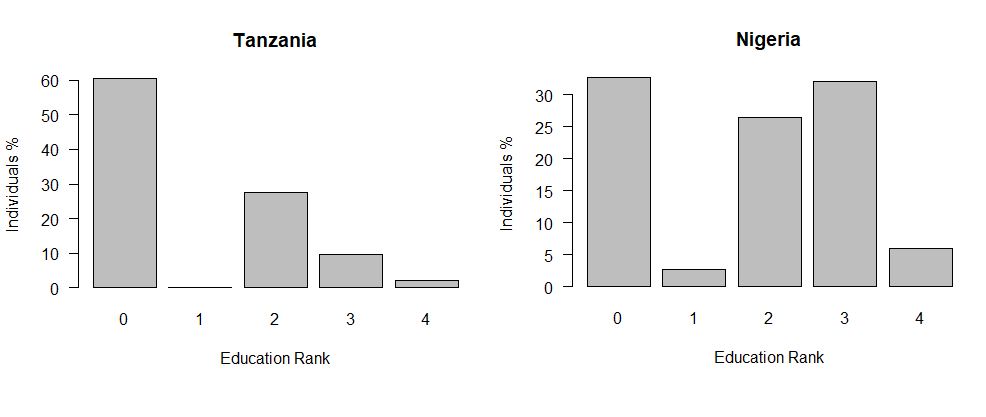
\includegraphics[width=6in]{figures/tnz_ngr_educranks2014-2015}
\par\end{centering}
\caption{\label{fig:HistEducationRanks}Education ranks for populations in
Tanzania and Nigeria (2012)}
\end{figure}

\begin{figure}
\begin{centering}
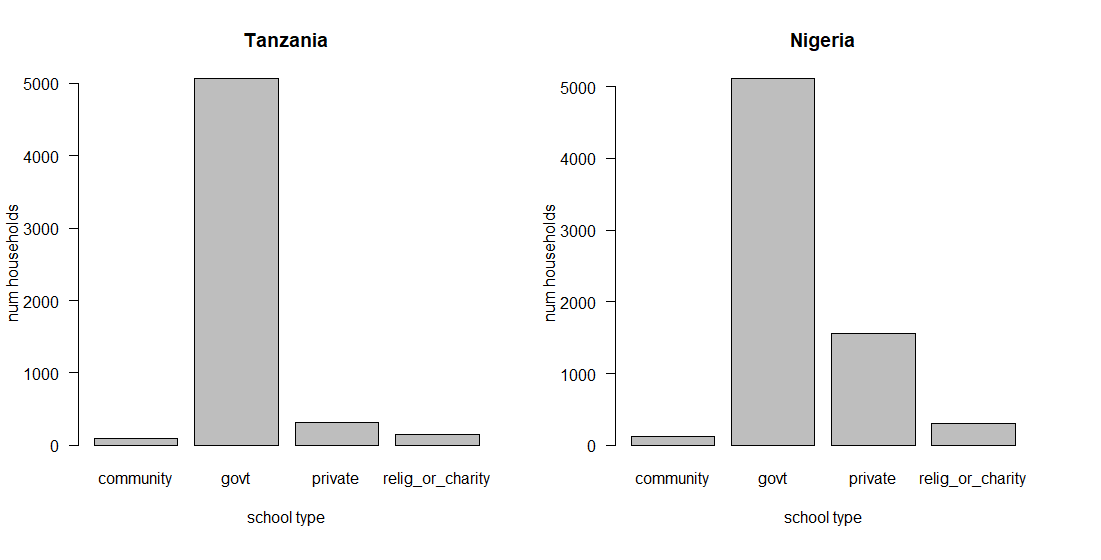
\includegraphics[width=6in]{figures/tnz_ngr_schooltype2012}
\par\end{centering}
\caption{\label{fig:BarChartSchoolTypes}School types for non-adult population
in Tanzania and Nigeria (2012)}
\end{figure}

\begin{figure}
\begin{centering}
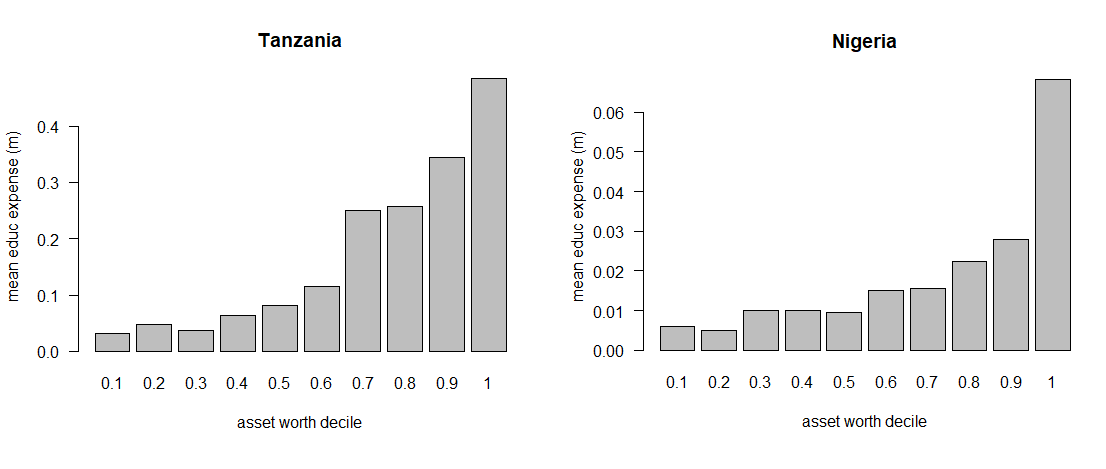
\includegraphics[width=6in]{figures/tnz_ngr_toteducexpense2012}
\par\end{centering}
\caption{\label{fig:BarChartEducationbyAssetDeciles}Educational expenses averages
over deciles of asset worth in in Tanzania and Nigeria (2012)}
\end{figure}

% Getting rural vs urban average expenditures 
% ddply(tn$df2012 [,c("hhid2012","toteducexpense","isrural")],.(isrural),summarise,toteducexpense=mean(toteducexpense))
% Getting children's education-rank averages
% ced <- merge(unique(subset(o2012,age<18  & !is.na(highest_educ))[c("hhid","education_rank")]),unique(plyr::rename(tn$df2012,c("hhid2012"="hhid"))[,c("hhid","toteducexpense")]))
% ddply(ced,.(education_rank),summarise,toteducexpense2=mean(toteducexpense), n=length(toteducexpense))

\noindent

Considering the overall distribution of education expenses, we see
that the urban residents spend much higher on education than the rural
residents in both the economies. More specifically, urban residents
spend 2.34 times more than rural residents in Nigeria whereas they
spend 2.8 times more in Tanzania. The secondary education appears
to get much costlier in Tanzania since the mean education expenditure
for education rank 3 (taken across all individuals with less than
18 age with education rank is almost double that of the expenditure
on education rank 2 in Tanzania. In Nigeria, these expenditures rise
by about 54\%. The educational expenses do not seem to rise much with
asset disparities in Nigeria - whereas they seem to be more unequally
distributed in Tanzania (see Figure \ref{fig:BarChartEducationbyAssetDeciles}).
Comparing education levels of the household heads, we see that the
average-education rank of the household heads in Tanzania (1.8) is
lower than that in Nigeria(1.9). We also see that the role of private
education is much higher in Nigeria (see Figure \ref{fig:BarChartSchoolTypes}).

The overall distribution of assets (durable goods stocks) in the two
countries is disparate. Contrasting the Lorenz curves for total non-durable
expenditure and total assets in the Figure \ref{fig:LorenzCurves}
for in Nigeria and Tanzania, we note that distribution of assets is
more sparse in Tanzania even though the overall expenditure appears
similarly distributed in the two countries.

A geographical distribution of assets further details that higher-income
occupations are far fewer in the hinterland and the southern regions
of Tanzania (see Figure \ref{fig:occupations_r_tn} ) - relative to
the eastern and coastal regions that seem largely urban. The disparities
in occupations are less in Nigeria (see Figure \ref{fig:occupations_r_ngr}
).

\begin{figure}[h]
\begin{centering}
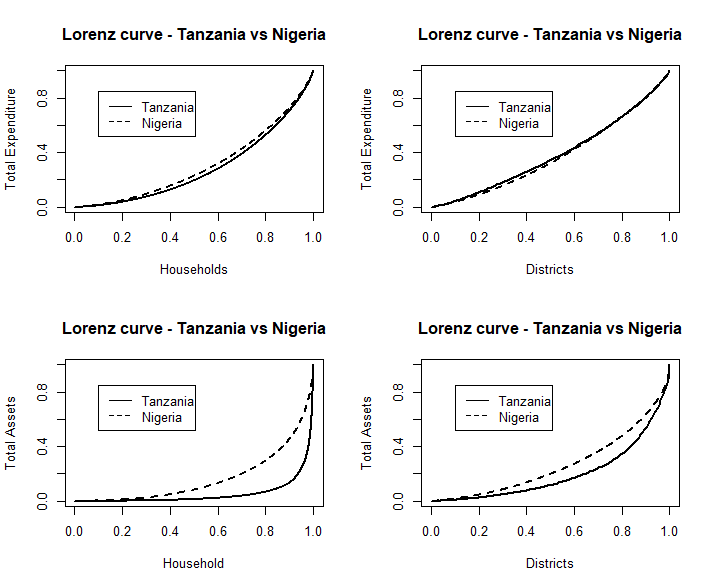
\includegraphics[width=3.75in]{figures/tnz_ngr_lorenz_curves_assets_logx_district_individual}
\par\end{centering}
\caption{\label{fig:LorenzCurves}Inequality in assets and non-durable expenditure
across households and districts}
\end{figure}

\onecolumn

\begin{figure}[h]
\begin{centering}
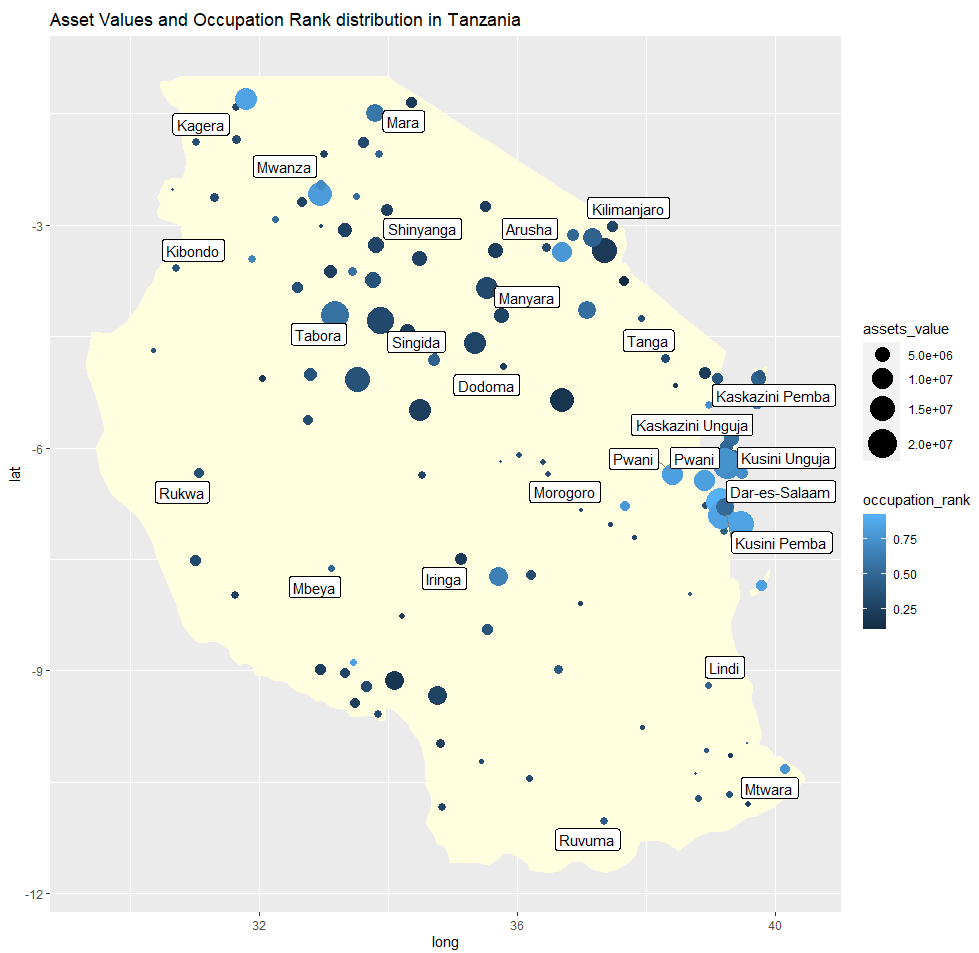
\includegraphics[width=3in]{tnz_assets_occuprank_distribution_2012}
\par\end{centering}
\caption{\label{fig:occupations_r_tn}Occupations and consumer-owned assets
in Tanzania}
\end{figure}

\begin{figure}[h]
\begin{centering}
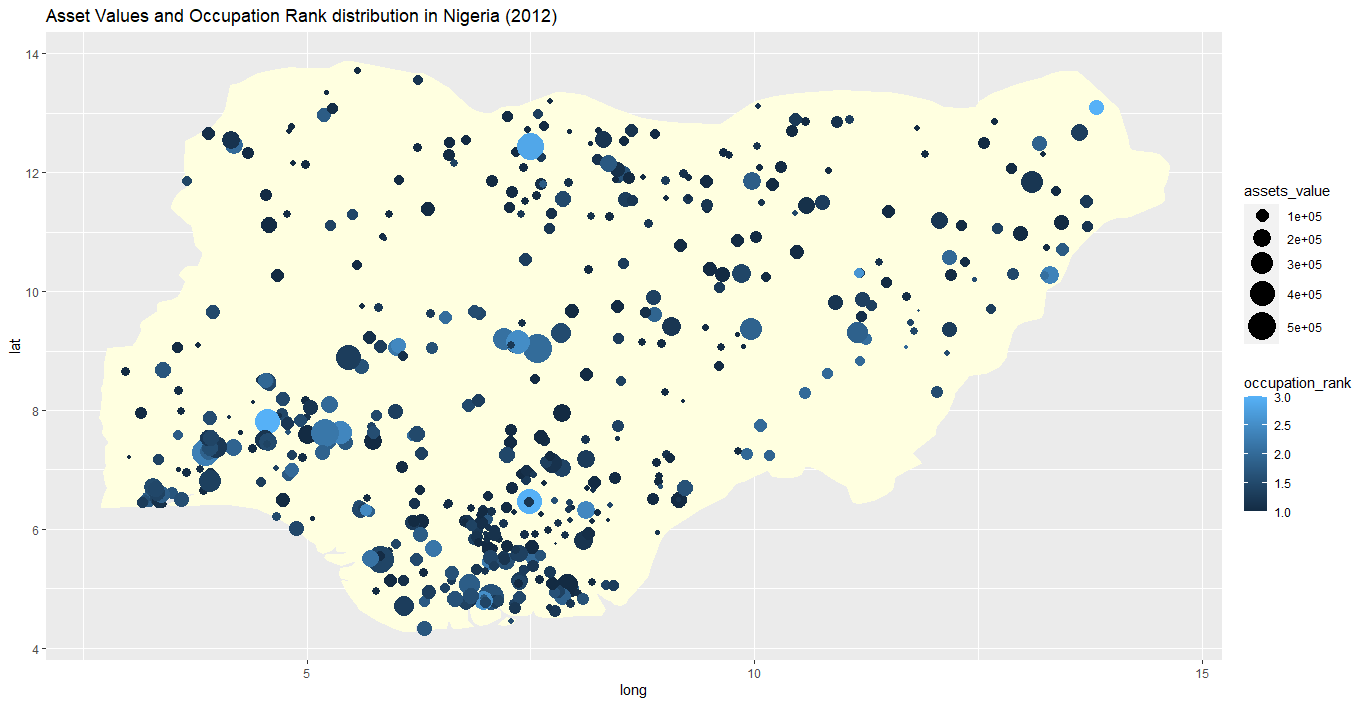
\includegraphics[width=4in]{ngr_occup_2012}
\par\end{centering}
\caption{\label{fig:occupations_r_ngr}Occupations and consumer-owned assets
in Nigeria}
\end{figure}

The occupation ranks shown in Figures \ref{fig:occupations_r_tn}
(Tanzania) and Figure \ref{fig:occupations_r_ngr} (Nigeria) are based
on the standardisation of various occupations in Tanzania and Nigeria.
Since the range of occupations in the surveys from Tanzania and Nigeria
is varied, the different occupations in the survey for Tanzania and
Nigeria have been standardised into occupation ranks (ranging from
0 to 3) based on the data on income derived from the occupations in
the survey so that a higher occupation rank represents an occupation
that provides higher income. The reason why the income itself is not
shown in the plots is that the data on income is far sparser than
the recall of assets and reporting of occupations in the surveys from
both the countries\footnote{It is not uncommon for the empirical studies in SSA to have the data
on occupation or education proxy the income differences (Alesina et
al.\cite{AlesinaMobilityAfrica2019}). The primary reason for this
is the sparsity of income data - a problem that may be further aggravated
because of a large informal sectors in the economies.}. The mapping from specific occupations to the occupation-ranks for
Tanzania and Nigeria is shown in Table \ref{occupation_rank_tn} and
\ref{occupation_rank_ngr} (respectively). A higher occupation rank
represents occupations that bring higher income. As described in Section
\ref{sec:Data}, the education levels are also mapped to education
ranks denoting primary, secondary and higher education (see Table
\ref{education_rank_tnz} for Tanzania and Table \ref{education_rank_ngr}
for Nigeria in the Appendix). A higher education rank corresponds
to a higher education level.

While we undertake a more detailed view on education expenses in the
Section \ref{subsec:Results}, the key observation from the data is
that the disparities in income and durable goods are more localised
in Nigeria while they are more extreme across wider geographical regions
in Tanzania. More specifically, despite the southern areas of Nigeria
having more higher-paid occupations and a higher expenditure on non-durable
expenditure overall (see Figure \ref{fig:occupations_r_ngr}), the
disparity in durable-goods ownership across regions is not as extreme
as in Tanzania. The particular interpretation of urbanisation is used
to explain the implications of this non-uniformity on consumption
and educational expenses in Section \ref{subsec:Results}.

% Lorenz curve plots
%plot(Lc(exp(ng$df2015$logx)))
% for individual totexp
%lorenz_curve(dat_a = exp(tn2012$logx),dat_b = exp(ng$df2012$logx),dat_a_name = "Tanzania",dat_b_name = "Nigeria",xlab = "Households",ylab = "Total Expenditure",use_cex = 1.)
% for district level totexp
%lorenz_curve(dat_a = exp(district_means(dat=tn2012,hhid_col = "hhid2012",field_type = "logx")$mean_logx),dat_b = exp(district_means(dat=ng$df2012,hhid_col = "hhid",field_type = "logx")$mean_logx),dat_a_name = "Tanzania",dat_b_name = "Nigeria",xlab = "Districts",ylab = "Total Expenditure",use_cex = 1.)
% for district level assets
%lorenz_curve(dat_a = exp(district_means(dat=tn2012,hhid_col = "hhid2012",field_type = "logA")$mean_logA),dat_b = exp(district_means(dat=ng$df2012,hhid_col = "hhid",field_type = "logA")$mean_logA),dat_a_name = "Tanzania",dat_b_name = "Nigeria",xlab = "Districts",ylab = "Total Assets",use_cex = 1.)
% For individual assets
%lorenz_curve(dat_a = exp(tn2012$logA),dat_b = exp(ng$df2012$logA),dat_a_name = "Tanzania",dat_b_name = "Nigeria",xlab = "Household",ylab = "Total Assets",use_cex = 1.)


\subsection{\label{subsec:Results}Results}

% We don't have panel information for 2012-2014 (for Tanzania). So we won't be using panel data. Pseudo-panel is a possibility but not considered.

\noindent

The two dependent variables we use in the estimation described in
Section \ref{sec:Econometric-Method} (see Equation \ref{eq:budgetshr_estimation})
are the budget shares for educational expenses (\texttt{$w_{educ}$})
and total expenditures (\texttt{$log(x_{educ})$}) . These dependent
variables are listed in Table \ref{tab:Dependent Variables} while
controls used for the estimation are listed in Table \ref{tab:Control-Variables}
.

%Variables : {wealth,wealth-conc/ruralwards,secondary_schools,occupation, parental education, language-religion, age, numchild, educpriv}

The two main explanatory variables used in the study are the private
household income (measured as the logarithm of total expenditure \texttt{ln\_tot\_exp})
and the urbanisation levels (measured as wealth-concentration \texttt{assetdensity}).
As discussed before, an alternative formulation is also specified
for comparison - where the two explanatory variables are the logarithm
of total assets value (\texttt{ln\_tot\_assets}) and the urban/rural
indicators (\texttt{rural\_wards}). The physical access to education
(i.e. \texttt{secondary\_schools}) is an important control in both
the formulations. Other controls used in the comparison are the indicator
for an agrarian occupation \texttt{agri} ($\Omega$), the paternal
education level \texttt{highesteduc} ($\Gamma^{*}$), the religion
and language indicators ( \texttt{religion} $\chi$ used only for
Nigeria indicated by 1 for Christianity, 2 for Islam, 3 for Traditional,
4 for other - and english-speaking ability i.e. the variable \texttt{has\_english
$\xi$ }indicating the ability to speak English used only for Tanzania),
the access to private education (\texttt{educpriv} or $\pi$), the
number of children ( \texttt{numchild} or $h$) and their ages \texttt{is\_primaryage}
($\mu_{1}$),\texttt{ is\_secondaryage} ($\mu_{2}$)\texttt{, is\_tertiaryage}
($\mu_{3})$ indicating if they are eligible (due to age) for primary,
secondary or tertiary education (respectively) and the non-durable
consumption prices \texttt{\small{}(log\_mean\_cost\_ne} $p_{ne}$).
All of the controls remain the same for the main as well as alternative
formulation. Recall that the non-durable consumption prices $p_{ne}$
(see Section \ref{sec:Data}) - interpreted as the cost of living
in the vicinity - is measured as the average consumption excluding
the asset-related costs in the consumer's vicinity. Notice that the
factor variables are prefixed with respective values \texttt{1.} ,
\texttt{2.} etc. in the results.

Of the control variables and explanatory variables discussed above,
some are observed at the household level while others are observed
at the level of the consumer's district. The logarithm of total expenditure
\texttt{ln\_tot\_exp} and of the total assets-owned \texttt{ln\_tot\_assets}
are observed at the level of the household. Similarly, the agricultural-occupation
factor variable \texttt{agri} (indicating whether the household head
is employed in agriculture related occupation or not), the number
of children in the household \texttt{numchild}, the childrens' ages
factor variables \texttt{is\_primaryage} ,\texttt{ is\_secondaryage}
and \texttt{is\_tertiaryage} ), the private education factor variable
\texttt{educpriv}, the highest education rank \texttt{highesteduc}
corresponding to the paternal generations (father-relationship) in
a household, the ability to speak English \texttt{has\_english} (used
only for Tanzania) and the household religion \texttt{religion} (used
only for Nigeria) are all observed for a household. The variables
observed at the district (or 6-$km$ vicinity) are the number of wards
with an accessible (within 6-km distance) secondary-schools (\texttt{secondary\_schools}),
the rural wards (\texttt{\small{}rural\_wards}) in a district, the
respective measures of the wealth-concentration \texttt{\small{}assetdensity}
and the logarithm of the per-head cost non-durable consumption \texttt{\small{}log\_mean\_cost\_ne}
.

To reiterate, a significant number of household units in both the
economies are made up of joint families where the reported educational
expenses correspond to the grandchildren of the household head (HH).
The education level of the HH would thus point to the penultimate
generation for households where HH has grandchildren and the previous
generation for younger households where HH has young children. To
resolve this disparity, we avoid using the education rank of the HH
and instead use the highest education rank in the generation of the
students' parents \footnote{Only relations with the household head are reported in the survey.
Thus, there is no direct way of locating the parent of a child except
through the relation with the household-head.} \texttt{\small{}highesteduc} instead. The paternal educational level
\texttt{\small{}highesteduc} suffices for the analysis of expenditure
spent over all the children in the household (rather than how education
budget is distributed among the children). As mentioned in the Section
\ref{sec:Econometric-Method}, the households with no children are
ignored in the analysis. Nearly 22\% of households in the Nigeria
and 15 \% of households in Tanzania are thus excluded from our comparison.

Notice also that the age-variables \texttt{is\_primaryage}, \texttt{is\_secondaryage},
\texttt{is\_tertiaryage} for attendance of primary, secondary and
tertiary education have been used in the analysis to get around the
unavailability of the current-education level of the household member
in the Nigerian LSMS survey data. Instead, we use a combination of
the indicator variable telling whether a household member is in school
or not (available in the surveys for both Tanzania and Nigeria) and
the mean school attendance ages to define variables \texttt{is\_primaryage},
\texttt{is\_secondaryage} and \texttt{is\_tertiaryage} that indicate
whether there is a household member of an age appropriate for attending
primary, secondary and tertiary education levels (respectively).

% For Nigeria: length(unique(subset(ng$df2015,toteducexpense==0)$hhid))/length(unique(ng$df2015$hhid)) = .67493
% For Tanzania: length(unique(subset(tn$df2014,toteducexpense==0)$hhid))/length(unique(tn$df2014$hhid)) = .4215

The results from the a tobit estimation for educational expenses (\texttt{$w_{educ}$})
and total expenditures (\texttt{$log(x_{educ})$}) with wealth-concentration
\texttt{assetdensity} as one of the controls are shown in Table \ref{tabTNZNGR_r}
for both Tanzania and Nigeria. The tobit uses a lower limit of zero
given a number of houses have no expenditure on education. More particularly,
a zero expenditure is reported for nearly 65\% households in the survey
from Nigeria (2015) and 43\% households in the survey from Tanzania
(2014). A discussion on the cross-section results from the latest
available years 2014 for Tanzania and 2015 for Nigeria follows in
Section \ref{subsec:Discussion}. The results from the alternative
formulation - where the main explanatory variables are the logarithm
of total assets value \texttt{\small{}ln\_tot\_assets} (used in place
of household total expenditure ) and the ruralness-score \texttt{\small{}rural\_wards
}derived from the survey's classificaiton of rural and urban areas
(used in place of wealth concentration \texttt{\small{}assetdensity}
) - are presented in Table \ref{tabTNZNGR_urbanrural}.

\subsection{\label{subsec:Discussion}Discussion}

%[secondary_schools effect]
%For Nigeria, the secondary-schools were split into community and government schools - whose sum turns out to be less than the schools recorded in the previous year. This seems to the cause of some disparity in the two years - even though the effect of this variable does not appear as significant as wealth.
% NGR:
% a<- merge(ddply(unique(subset(ng$df2012[,c("region","district","secondary_schools")],!is.na(secondary_schools))),.(region),summarise,n=sum(secondary_schools)), ddply(unique(subset(ng$df2015[,c("region","district","secondary_schools")],!is.na(secondary_schools))),.(region),summarise,n=sum(secondary_schools)), by =c("region"))
% b<- merge(ddply(unique(subset(tn$df2012[,c("region","district","secondary_schools")],!is.na(secondary_schools))),.(region),summarise,n=sum(secondary_schools)), ddply(unique(subset(tn$df2014[,c("region","district","secondary_schools")],!is.na(secondary_schools))),.(region),summarise,n=sum(secondary_schools)), by =c("region"))
%[secondary_schools effect]


\noindent

%[ln_tot_exp effect on budget share]

The results in Tables \ref{tabTNZNGR_r} suggest that an increase
in the total expenditure ( \texttt{ln\_tot\_exp)} causes a decrease
in the budget share on education \texttt{$w_{educ}$} for both Tanzania
and Nigeria. This seems largely due to the educational expenses forming
a higher proportion of the total expenditure for poorer households
- since the education expenditures do seem to rise with the increase
in total expenditure in Tanzania if one views the results with education-expenditure
logarithm \texttt{$log(x_{educ})$ }as the dependent variable (see
further discussion of the results from estimation with education-expenditure
as dependent variable). The effect of non-durable consumption prices
(\texttt{log\_mean\_cost\_ne} ) is weak on education-budget share
\texttt{$w_{educ}$} for both the economies. Thus while urbanisation
must raise the prices of non-durable expenditure excluding asset-costs
\texttt{log\_mean\_cost\_ne}, the disparity in budget shares does
not appear to be due to higher cost of living (non-durable consumption)
alone.

%[r - w_educ]

Instead, we see a strong and positive effect of wealth concentration
( \texttt{assetdensity} ) towards educational budget shares (\texttt{$w_{educ}$})
in both the countries in Table \ref{tabTNZNGR_r}. The effects of
household income are relevant - however - for private education -
which is limited to the wealthier households in both the economies
regardless of wealth-concentration ( \texttt{assetdensity} ). Private
education is slightly more important in Nigeria (see Figure \ref{fig:BarChartSchoolTypes})
as the privately-educated households in Nigeria show higher budget
shares \texttt{$w_{educ}$ }for education (see Table \ref{tabTNZNGR_r}
). Since private education only accounts for a minority of the population
in both the economies (see Figure \ref{fig:BarChartSchoolTypes}),
the role of access to either or private or government secondary school
i.e. the variable \texttt{secondary\_schools} turns out to be more
important for our comparison of education expenses in the two countries.

Viewing the effect of the variable \texttt{secondary\_schools} on
education budget shares \texttt{$w_{educ}$}, we see a far stronger
effect of \texttt{secondary\_schools} for Tanzania (compare the coefficients
for secondary-school $s$ i.e. \texttt{secondary\_schools }in Tables
\ref{tabTNZNGR_r}) . It also seems that the consumers are more likely
to spend on primary education in Tanzania - as the attendance for
secondary and tertiary-education remains much lower (this is further
elaborated in discussion below of the results using education expenditure
\texttt{$log(x_{educ})$} as dependent variable).

Notice that results from the alternative formulation using urban-rural
indicators suggest a particular limitation of the use of urban-rural
indicators from the survey. The coefficients of rural-wards \texttt{(rural\_wards})
for education budget shares \texttt{$w_{educ}$} are negative and
significant for Tanzania in Table \ref{tabTNZNGR_urbanrural}. But
the inference of a higher expenditure on education - when using urban-rural
indicators - by the rural residents in Nigeria (see significance of
rural-wards \texttt{rural\_wards }in Table \ref{tabTNZNGR_urbanrural}
) ignores the fact that the wards identified as rural in Nigeria may
not be as rural as those identified as rural in Tanzania. This is
confirmed with the weaker role of wealth i.e. assets-worth-logarithm
( \texttt{ln\_tot\_assets} in Table \ref{tabTNZNGR_urbanrural}) and
a strong role for wealth-concentration (\texttt{assetdensity} in Table
\ref{tabTNZNGR_r}) for Nigeria in the alternative formulation. The
wealth-concentration \texttt{assetdensity} thus provides a more clear-cut
and standardised interpretation of urbanisation in the two economies
than what may be possible with the survey's urban-rural classifications.

%[log(x_educ)]

Comparing the results with education-expenditure logarithm \texttt{$log(x_{educ})$
}as the dependent variable, we see that the education expenditures
rise with the increase in total expenditure logarithm (\texttt{ln\_tot\_exp})
for Tanzania but the effect of income (the logarithm of total expenditure
\texttt{\small{}ln\_tot\_exp} in Table \ref{tabTNZNGR_r}) is not
significant for Nigeria. While the higher expenditure on education
measured through total education expenditure logarithm \texttt{$log(x_{educ})$}
does seem to correspond to the prices of non-durable consumption \texttt{log\_mean\_cost\_ne}
in Tanzania, the higher budget share of education cannot be attributed
to higher consumption-prices - since the effect of non-durable consumption
prices \texttt{log\_mean\_cost\_ne} remains weak on education-budget
share \texttt{$w_{educ}$} for both the economies (see above discussion
using budget share \texttt{$w_{educ}$} as the dependent variable).
Considering the effect of the second explanatory variable - the wealth
concentration ( \texttt{assetdensity} ) - we see a rise in educational
expenditure \texttt{$log(x_{educ})$} for Nigeria while the effect
of wealth concentration \texttt{assetdensity} is insignificant for
Tanzania (compare coefficients for \texttt{assetdensity} against both
the countries in Table \ref{tabTNZNGR_r}). In the alternative formulation
where urbanisation is measured with the ruralness score ( \texttt{rural\_wards}
), the ruralness score corresponds to a rise in educational expenditure
\texttt{$log(x_{educ})$} for Nigeria and a drop in educational expenditure
\texttt{$log(x_{educ})$ }for Tanzania (see Table \ref{tabTNZNGR_urbanrural}). 

Continuing with the comparison of results with education-expenditure
as the dependent variable, we see that private-education indicator
variable \texttt{educpriv} is insignificant for Nigeria (see Table
\ref{tabTNZNGR_r} ). It again seems evident that the attendance for
secondary and tertiary-education remains much lower in Tanzania (see
coefficients of secondary-school-age\texttt{ is\_secondaryage} and
tertiary-school-age \texttt{is\_tertiaryage} in regression results
with education expenditure logarithm $log(x_{educ})$ as the dependent
variable in Table \ref{tabTNZNGR_r}). In the alternative formulation,
the results with education expenditure logarithm \texttt{$log(x_{educ})$
}as dependent variable in Tables \ref{tabTNZNGR_urbanrural} show
the role of secondary-school access \texttt{secondary\_schools} to
be stronger for Nigeria when taking wealth i.e. total assets-worth
logarithm \texttt{ln\_tot\_assets }into account. The wealth effect
thus seems stronger than access in both the economies but is weaker
for Nigeria where more household members enroll into secondary and
tertiary education - regardless of the differences in long-term intergenerational
wealth (measured with logarithm of assets-worth \texttt{ln\_tot\_assets}).
The decomposed view of expenses on education in terms of secondary
and primary education level further clarifies this observation - reflecting
the far lower attendance of secondary education in Tanzania. 

The role of the number of children (\texttt{numchild}) also seems
stronger in Tanzania than in Nigeria - but the effect is likely due
the education expenses primarily driven by the primary education levels
in Tanzania (as well as a higher percentage of households reporting
no education expenditure in the survey from Nigeria). Another consequence
of most households spending on primary education alone is that the
agrarian households appear as spending higher on education after considering
the wealth-concentration among households with the same educational-status.
The education expenditure is higher for agrarian households in Tanzania
after taking into account their poor educational status measured through
$\Gamma$ (see coefficients of agrarian-occupation-indicator \texttt{1.is\_agri}
in Table \ref{tabTNZNGR_r} for education-expenditure-logarithm \texttt{$log(x_{educ})$}
as the dependent variable).

The wealth effects in Tanzania overall seem stronger, but they ought
to be considered in light of the much lower enrollment levels in secondary
(and higher) education and higher disparity in asset-ownership (even
after taking into account the lower urbanisation levels) in Tanzania.
The significance of logarithm of assets-worth ( \texttt{ln\_tot\_assets
}in Table \ref{tabTNZNGR_urbanrural}) does indicate a general trend
where those with higher inter-generational wealth and in urban areas
are far more likely to avail the education facilities, but a higher
dependence on industrial output in Nigeria also seems to have contributed
to a higher demand for secondary and tertiary education in the economy.
Another observation - the stronger role of father's education level
in Tanzania - also seems related with these disparities in the two
economies. A comparison of education expenditures across the two countries
must take into account the different stages which the two countries
appear to be in terms of urbanisation and economic development.

It is worth highlighting that the role of social environment is significant
in both the economies. The role of English language seems significant
in Tanzania - where the English-speakers spend significantly higher
on education. In Nigeria, on the other hand, the educational expenses
are higher among households identifying as Christian. In both cases,
the role of social characteristics seems rather inseparable from the
institutional differences towards education. In case of Tanzania,
the ability to speak English is aligned with attending educational
institutions while in Nigeria, the role played by Christian missionaries
in establishment of educational may be reflected in the disparity
of access to educational facilities.

\begin{table}\centering
\caption{Tanzania -Nigeria - Differences in Wealth Concentration  \label{tabTNZNGR_r}}
\resizebox{4in}{!}{
\def\sym#1{\ifmmode^{#1}\else\(^{#1}\)\fi}     
\begin{tabular} { l c c  c c }
\hline\hline       

          &\multicolumn{2}{c}{$w_{educ}$}       &\multicolumn{2}{c}{$log(x_{educ})$}  \\\cmidrule(lr){2-3}\cmidrule(lr){4-5}           &\multicolumn{1}{c}{}&\multicolumn{1}{c}{}&\multicolumn{1}{c}{}&\multicolumn{1}{c}{}\\           &\multicolumn{1}{c}{\emph{Tanzania}}&\multicolumn{1}{c}{\emph{Nigeria}}&\multicolumn{1}{c}{\emph{Tanzania}}&\multicolumn{1}{c}{\emph{Nigeria}}\\ \midrule ln\_tot\_exp      & -0.00908\sym{**} &  -0.0283\sym{***}&    1.224\sym{***}&    0.133         \\           &  (0.004)         &  (0.000)         &  (0.000)         &  (0.744)         \\ assetdensity     &  0.00488\sym{*}  &   0.0299\sym{***}&  -0.0368         &    1.497\sym{***}\\           &  (0.015)         &  (0.000)         &  (0.758)         &  (0.000)         \\ log\_mean\_cost\_ne&   0.0490         &   0.0479         &    9.165\sym{*}  &   -0.155         \\           &  (0.467)         &  (0.672)         &  (0.023)         &  (0.981)         \\ 1.agri    &  0.00735         &  0.00990         &    0.953\sym{**} &    0.574         \\           &  (0.167)         &  (0.308)         &  (0.003)         &  (0.297)         \\ 1.educpriv&   0.0756\sym{***}&   0.0475\sym{***}&    2.890\sym{***}&    0.815         \\           &  (0.000)         &  (0.000)         &  (0.000)         &  (0.197)         \\ 1.highesteduc&   0.0109\sym{*}  &   0.0829         &    0.694\sym{*}  &    5.899         \\           &  (0.030)         &  (0.301)         &  (0.021)         &  (0.202)         \\ 2.highesteduc&  0.00432         &  0.00679         &    0.366         &    0.363         \\           &  (0.711)         &  (0.585)         &  (0.598)         &  (0.607)         \\ 3.highesteduc&  0.00457         & -0.00520         &    0.473         &   -0.528         \\           &  (0.519)         &  (0.627)         &  (0.263)         &  (0.381)         \\ 4.highesteduc&   0.0250\sym{*}  &   0.0120         &    1.465\sym{*}  &    0.183         \\           &  (0.011)         &  (0.506)         &  (0.013)         &  (0.859)         \\ secondary\_schools& -0.00138\sym{***}&  0.00738         & -0.00569         &    0.384         \\           &  (0.000)         &  (0.373)         &  (0.734)         &  (0.414)         \\ 1.is\_primaryage&   0.0793\sym{***}&   0.0538\sym{***}&    8.842\sym{***}&    3.301\sym{***}\\           &  (0.000)         &  (0.000)         &  (0.000)         &  (0.000)         \\ 1.is\_secondaryage&   0.0123\sym{**} &   0.0605\sym{***}&    0.143         &    2.230\sym{***}\\           &  (0.005)         &  (0.000)         &  (0.580)         &  (0.000)         \\ 1.is\_tertiaryage&  -0.0131\sym{**} &   0.0174         &   -1.281\sym{***}&    0.931         \\           &  (0.001)         &  (0.056)         &  (0.000)         &  (0.071)         \\ 1.has\_english&   0.0584\sym{***}&                  &    2.249\sym{***}&                  \\           &  (0.000)         &                  &  (0.000)         &                  \\ numchild  &  0.00433\sym{***}& -0.00221         &    0.259\sym{***}&  -0.0499         \\           &  (0.000)         &  (0.360)         &  (0.000)         &  (0.714)         \\ 2.religion&                  &  -0.0455\sym{***}&                  &   -2.043\sym{***}\\           &                  &  (0.000)         &                  &  (0.000)         \\ 3.religion&                  &  -0.0632         &                  &   -2.160         \\           &                  &  (0.170)         &                  &  (0.396)         \\ \_cons    &   -0.151         &   -0.231         &   -41.97\sym{***}&   -22.99         \\           &  (0.346)         &  (0.352)         &  (0.000)         &  (0.103)         \\ \midrule sigma     &                  &                  &                  &                  \\ \_cons    &   0.0876\sym{***}&    0.173\sym{***}&    5.361\sym{***}&    9.969\sym{***}\\           &  (0.000)         &  (0.000)         &  (0.000)         &  (0.000)         \\ \midrule \(N\)     &     2410         &     2192         &     2410         &     2192         \\ 

\end{tabular}
}
\end{table}

\begin{table}\centering
\caption{Tanzania-Nigeria - Urban-Rural Differences \label{tabTNZNGR_urbanrural}}
\resizebox{4in}{!}{
\def\sym#1{\ifmmode^{#1}\else\(^{#1}\)\fi}     
\begin{tabular} { l c c  c c }
\hline\hline       

          &\multicolumn{2}{c}{$w_{educ}$}       &\multicolumn{2}{c}{$log(x_{educ})$}  \\\cmidrule(lr){2-3}\cmidrule(lr){4-5}           &\multicolumn{1}{c}{}&\multicolumn{1}{c}{}&\multicolumn{1}{c}{}&\multicolumn{1}{c}{}\\           &\multicolumn{1}{c}{\emph{Tanzania}}&\multicolumn{1}{c}{\emph{Nigeria}}&\multicolumn{1}{c}{\emph{Tanzania}}&\multicolumn{1}{c}{\emph{Nigeria}}\\ \midrule ln\_tot\_assets      & -0.00590\sym{***}& -0.00196         &    0.392\sym{***}&    0.363         \\           &  (0.000)         &  (0.576)         &  (0.000)         &  (0.065)         \\ log\_mean\_cost\_ne&  -0.0548         & -0.00483         &    9.559\sym{*}  &    8.263         \\           &  (0.455)         &  (0.965)         &  (0.031)         &  (0.182)         \\ 1.agri    &   0.0106\sym{*}  &  0.00507         &    0.925\sym{**} &  -0.0768         \\           &  (0.048)         &  (0.617)         &  (0.004)         &  (0.892)         \\ 1.educpriv&   0.0800\sym{***}&   0.0506\sym{***}&    2.730\sym{***}&    1.016         \\           &  (0.000)         &  (0.000)         &  (0.000)         &  (0.113)         \\ 1.highesteduc&   0.0107\sym{*}  &   0.0948         &    0.679\sym{*}  &    7.172         \\           &  (0.032)         &  (0.244)         &  (0.023)         &  (0.121)         \\ 2.highesteduc&  0.00199         &  0.00689         &    0.512         &    0.481         \\           &  (0.864)         &  (0.583)         &  (0.462)         &  (0.495)         \\ 3.highesteduc&  0.00359         & -0.00767         &    0.607         &   -0.551         \\           &  (0.608)         &  (0.478)         &  (0.149)         &  (0.361)         \\ 4.highesteduc&   0.0273\sym{**} &   0.0129         &    1.320\sym{*}  &    0.486         \\           &  (0.005)         &  (0.480)         &  (0.025)         &  (0.636)         \\ secondary\_schools& -0.00111\sym{***}&   0.0147         &  0.00265         &    0.906         \\           &  (0.000)         &  (0.085)         &  (0.875)         &  (0.058)         \\ 1.is\_primaryage&   0.0797\sym{***}&   0.0562\sym{***}&    8.812\sym{***}&    3.408\sym{***}\\           &  (0.000)         &  (0.000)         &  (0.000)         &  (0.000)         \\ 1.is\_secondaryage&   0.0129\sym{**} &   0.0593\sym{***}&    0.145         &    2.259\sym{***}\\           &  (0.003)         &  (0.000)         &  (0.572)         &  (0.000)         \\ 1.is\_tertiaryage&  -0.0121\sym{**} &   0.0139         &   -1.240\sym{***}&    0.878         \\           &  (0.003)         &  (0.132)         &  (0.000)         &  (0.088)         \\ rural\_wards&  -0.0229\sym{**} &   0.0133         &   -1.184\sym{*}  &    1.848\sym{**} \\           &  (0.007)         &  (0.291)         &  (0.021)         &  (0.009)         \\ 1.has\_english&   0.0599\sym{***}&                  &    2.436\sym{***}&                  \\           &  (0.000)         &                  &  (0.000)         &                  \\ numchild  &  0.00426\sym{***}& -0.00354         &    0.304\sym{***}&  -0.0588         \\           &  (0.000)         &  (0.143)         &  (0.000)         &  (0.662)         \\ 2.religion&                  &  -0.0445\sym{***}&                  &   -1.716\sym{**} \\           &                  &  (0.000)         &                  &  (0.003)         \\ 3.religion&                  &  -0.0725         &                  &   -2.411         \\           &                  &  (0.120)         &                  &  (0.343)         \\ \_cons    &    0.143         &   -0.103         &   -30.47\sym{**} &   -29.99\sym{*}  \\           &  (0.452)         &  (0.698)         &  (0.008)         &  (0.044)         \\ \midrule sigma     &                  &                  &                  &                  \\ \_cons    &   0.0870\sym{***}&    0.175\sym{***}&    5.357\sym{***}&    9.994\sym{***}\\           &  (0.000)         &  (0.000)         &  (0.000)         &  (0.000)         \\ \midrule \(N\)     &     2410         &     2192         &     2410         &     2192         \\ 

\end{tabular}
}
\end{table}

\bigskip{}

\begin{landscape}
\begin{table}\centering
\caption{Tanzania-Nigeria - around median assets-value \label{tabTNZNGR_abovebelow_median}}
\resizebox{7.5in}{!}{
\def\sym#1{\ifmmode^{#1}\else\(^{#1}\)\fi}     
\begin{tabular} { l c c  c c c c c c }
\hline\hline       

          &\multicolumn{2}{c}{$w_{educ}$}&\multicolumn{2}{c}{$log(x_{educ})$}&\multicolumn{2}{c}{$w_{educ}$}&\multicolumn{2}{c}{$log(x_{educ})$}\\\cmidrule(lr){2-3}\cmidrule(lr){4-5}\cmidrule(lr){6-7}\cmidrule(lr){8-9}           &\multicolumn{1}{c}{Above Median }&\multicolumn{1}{c}{Above Median }&\multicolumn{1}{c}{Above Median }&\multicolumn{1}{c}{Above Median }&\multicolumn{1}{c}{Below Median }&\multicolumn{1}{c}{Below Median }&\multicolumn{1}{c}{Below Median }&\multicolumn{1}{c}{Below Median }
\\           &\multicolumn{1}{c}{\emph{Tanzania}}&\multicolumn{1}{c}{\emph{Nigeria}}&\multicolumn{1}{c}{\emph{Tanzania}}&\multicolumn{1}{c}{\emph{Nigeria}}&\multicolumn{1}{c}{\emph{Tanzania}}&\multicolumn{1}{c}{\emph{Nigeria}}&\multicolumn{1}{c}{\emph{Tanzania}}&\multicolumn{1}{c}{\emph{Nigeria}}
\\ \midrule ln\_tot\_exp      & -0.00338         &  -0.0168         &    0.783\sym{**} &    0.411         &  -0.0121\sym{**} &  -0.0458\sym{***}&    1.272\sym{***}&   -0.582         \\           &  (0.483)         &  (0.113)         &  (0.005)         &  (0.511)         &  (0.006)         &  (0.000)         &  (0.000)         &  (0.321)         \\ assetdensity     &  0.00512         &   0.0321\sym{***}&   -0.160         &    1.818\sym{***}&  0.00592         &   0.0227\sym{*}  &  -0.0190         &    0.819         \\           &  (0.061)         &  (0.000)         &  (0.311)         &  (0.000)         &  (0.052)         &  (0.024)         &  (0.919)         &  (0.131)         \\ log\_mean\_cost\_ne&  -0.0900         & -0.00476         &    11.02         &   -6.579         &    0.165         &    0.100         &    7.127         &    5.568         \\           &  (0.363)         &  (0.976)         &  (0.056)         &  (0.479)         &  (0.080)         &  (0.539)         &  (0.219)         &  (0.528)         \\ 1.agri    &  0.00286         &  0.00554         &    0.758         &    0.341         &   0.0129         &   0.0157         &    1.151\sym{*}  &    0.809         \\           &  (0.671)         &  (0.665)         &  (0.052)         &  (0.650)         &  (0.139)         &  (0.294)         &  (0.031)         &  (0.314)         \\ 1.educpriv&   0.0850\sym{***}&   0.0348\sym{*}  &    3.219\sym{***}&    0.726         &   0.0527\sym{**} &   0.0711\sym{***}&    2.083         &    0.896         \\           &  (0.000)         &  (0.010)         &  (0.000)         &  (0.364)         &  (0.004)         &  (0.000)         &  (0.074)         &  (0.406)         \\ 1.highesteduc&   0.0102         &   0.0847         &    0.443         &    8.091         &   0.0118         &    0.107         &    0.850\sym{*}  &    5.336         \\           &  (0.156)         &  (0.482)         &  (0.292)         &  (0.263)         &  (0.089)         &  (0.323)         &  (0.047)         &  (0.368)         \\ 2.highesteduc&   0.0208         &  0.00761         &    0.759         &    0.178         &  -0.0235         &  0.00660         &   -0.380         &    0.618         \\           &  (0.170)         &  (0.645)         &  (0.390)         &  (0.855)         &  (0.207)         &  (0.727)         &  (0.735)         &  (0.543)         \\ 3.highesteduc&-0.000380         & -0.00517         &  -0.0789         &   -0.359         &   0.0114         & -0.00197         &    1.171         &   -0.594         \\           &  (0.967)         &  (0.711)         &  (0.882)         &  (0.661)         &  (0.310)         &  (0.906)         &  (0.092)         &  (0.508)         \\ 4.highesteduc&   0.0204         &  0.00328         &    0.796         &   -0.695         &   0.0368         &   0.0426         &    2.572\sym{*}  &    2.785         \\           &  (0.079)         &  (0.877)         &  (0.240)         &  (0.577)         &  (0.062)         &  (0.222)         &  (0.036)         &  (0.139)         \\ secondary\_schools& -0.00128\sym{***}& -0.00325         & -0.00576         &   -0.524         & -0.00161\sym{**} &   0.0230         &  0.00286         &    1.669\sym{*}  \\           &  (0.000)         &  (0.764)         &  (0.770)         &  (0.413)         &  (0.001)         &  (0.077)         &  (0.926)         &  (0.018)         \\ 1.is\_primaryage&   0.0610\sym{***}&   0.0465\sym{**} &    7.280\sym{***}&    2.766\sym{**} &    0.101\sym{***}&   0.0664\sym{***}&    10.53\sym{***}&    3.983\sym{***}\\           &  (0.000)         &  (0.003)         &  (0.000)         &  (0.003)         &  (0.000)         &  (0.000)         &  (0.000)         &  (0.000)         \\ 1.is\_secondaryage&  0.00978         &   0.0692\sym{***}&   0.0488         &    2.637\sym{***}&   0.0161\sym{*}  &   0.0502\sym{***}&    0.243         &    1.706\sym{*}  \\           &  (0.100)         &  (0.000)         &  (0.887)         &  (0.000)         &  (0.011)         &  (0.000)         &  (0.533)         &  (0.020)         \\ 1.is\_tertiaryage&  -0.0109\sym{*}  &   0.0152         &   -1.381\sym{***}&    0.727         &  -0.0151\sym{*}  &   0.0193         &   -1.311\sym{***}&    1.108         \\           &  (0.043)         &  (0.197)         &  (0.000)         &  (0.292)         &  (0.015)         &  (0.181)         &  (0.001)         &  (0.152)         \\ 1.has\_english&   0.0496\sym{***}&                  &    1.789\sym{***}&                  &   0.0704\sym{***}&                  &    2.575\sym{***}&                  \\           &  (0.000)         &                  &  (0.000)         &                  &  (0.000)         &                  &  (0.000)         &                  \\ numchild  &  0.00204         & -0.00315         &    0.267\sym{**} &   -0.115         &  0.00657\sym{***}& -0.00143         &    0.231\sym{*}  &   0.0342         \\           &  (0.167)         &  (0.307)         &  (0.002)         &  (0.523)         &  (0.000)         &  (0.713)         &  (0.027)         &  (0.870)         \\ 2.religion&                  &  -0.0439\sym{***}&                  &   -1.963\sym{*}  &                  &  -0.0466\sym{**} &                  &   -2.037\sym{*}  \\           &                  &  (0.001)         &                  &  (0.011)         &                  &  (0.003)         &                  &  (0.015)         \\ 3.religion&                  &   -0.121         &                  &   -6.104         &                  &  -0.0373         &                  &   -0.447         \\           &                  &  (0.144)         &                  &  (0.192)         &                  &  (0.516)         &                  &  (0.882)         \\ \_cons    &    0.145         &   -0.250         &   -36.11\sym{**} &   -13.01         &   -0.447         &   -0.103         &   -39.80\sym{**} &   -22.74         \\           &  (0.521)         &  (0.475)         &  (0.006)         &  (0.527)         &  (0.061)         &  (0.777)         &  (0.007)         &  (0.246)         \\ \midrule sigma     &                  &                  &                  &                  &                  &                  &                  &                  \\ \_cons    &   0.0861\sym{***}&    0.169\sym{***}&    5.114\sym{***}&    10.13\sym{***}&   0.0877\sym{***}&    0.176\sym{***}&    5.545\sym{***}&    9.644\sym{***}\\           &  (0.000)         &  (0.000)         &  (0.000)         &  (0.000)         &  (0.000)         &  (0.000)         &  (0.000)         &  (0.000)         \\ \midrule \(N\)     &     1233         &     1192         &     1233         &     1192         &     1177         &     1000         &     1177         &     1000         \\ 

\end{tabular}
}
\end{table}
\end{landscape} 

\noindent

\subsection{Robustness Checks}

\noindent

As a first robustness check, we re-estimate the results with wealth
concentration \texttt{assetdensity} as the explanatory variable for
those with less than the local median wealth i.e. assets-worth logarithm
\texttt{ln\_tot\_assets} and for those above it. The results demonstrate
how the education expenditures (coefficients for education budget-shares
\texttt{$w_{educ}$ }and education-expenditure logarithm \texttt{$log(x_{educ})$})
differ between the poorer and richer households in a given locality.
The results for above and below local median-assets possession using
education budget-shares \texttt{$w_{educ}$ }and education-expenditure-logarithm
\texttt{$log(x_{educ})$ }as the dependent variables are shown in
Table \ref{tabTNZNGR_abovebelow_median} for both above and below
median assets-possession levels in the two countries. 

%[Results from first robustness check ] social factors and secondary_schools . educpriv expected. tertiary_school level lower. num_child more nuanced - as is r. highesteduc also different.

The role of social effects seems validated with these results as the
significance of social factors remains unaffected by whether the consumers
have above or below the median asset ownership level. More specifically,
the factor variables for english-speaking ability \texttt{has\_english}
and (i.e. \texttt{religion }) are significant in results from Tanzania
and Nigeria (respectively) for both richer and poorer households.
The factor variable for english-speaking ability \texttt{has\_english}
is significant for consumers both above and below media asset possession
level (the coefficient for variable \texttt{religion }is significant
for Nigeria for above and below median asset possession level in Table
\ref{tabTNZNGR_abovebelow_median}). It is worth pointing out that
the economic significance for religion ( \texttt{religion }) in Nigeria
is higher with \texttt{$log(x_{educ})$} as dependent variable in
Table \ref{tabTNZNGR_abovebelow_median}. 

As one would expect, the effect of secondar-schools \texttt{secondary\_schools}
is also the same for both richer and poorer halves of a given locality.
While the role that the wealth-concentration \texttt{assetdensity}
plays towards access to education appears to be the same for the rich
and poor halves in a locality as well, we do see a higher economic
significance of wealth-concentration \texttt{assetdensity} for the
below-median-assets household in Nigeria - possibly because of high
education costs in urban areas where asset-possession may be lower.
The access to private education and to higher education favour the
richer households in both economies - as the economic significance
of private-education factor variable \texttt{educpriv }is consistently
higher for richer households as is the expenditure on tertiary level
education in both the economies.

The number of children have a more significant effect for richer households
in Tanzania. Given a lower participation in higher education in the
country, this effect seems likely due to the primary-education needs
scaling up with the number of children in the household. As in the
Section \ref{subsec:Discussion}, the lower levels of average educational
attainment in Tanzania seem to accentuate the effect of paternal education
rank \texttt{highesteduc }which has a higher statistical significance
for poorer households in Tanzania (compare the coefficient of paternal
education rank \texttt{highesteduc }in Tanzania with educational-expenditure
logarithm \texttt{$log(x_{educ})$} as dependent variable for both
above and below median assets possession level in Table \ref{tabTNZNGR_abovebelow_median})
whereas the significance is not much different for richer and poorer
households in Nigeria (see Table \ref{tabTNZNGR_abovebelow_median}).

\begin{table}\centering
\caption{Tanzania-Nigeria - $assetdensity_{educ}$ \label{tabTNZNGR_reduc}}
\resizebox{4in}{!}{
\def\sym#1{\ifmmode^{#1}\else\(^{#1}\)\fi}     
\begin{tabular} { l c c  c c }
\hline\hline
 

          &\multicolumn{2}{c}{$w_{educ}$}       &\multicolumn{2}{c}{$log(x_{educ})$}  \\\cmidrule(lr){2-3}\cmidrule(lr){4-5}           &\multicolumn{1}{c}{  \emph{Tanzania}}&\multicolumn{1}{c}{\emph{Nigeria}}&\multicolumn{1}{c}{\emph{Tanzania}}&\multicolumn{1}{c}{\emph{Nigeria}}\\
\midrule ln\_tot\_exp      & -0.00927\sym{**} &  -0.0291\sym{***}&    1.229\sym{***}&   0.0988         \\           &  (0.004)         &  (0.000)         &  (0.000)         &  (0.809)         \\ assetdensity\_educ &  0.00262         &   0.0272\sym{***}&  -0.0349         &    1.323\sym{***}\\           &  (0.102)         &  (0.000)         &  (0.714)         &  (0.000)         \\ log\_mean\_cost\_ne&   0.0535         &   0.0570         &    9.210\sym{*}  &    0.361         \\           &  (0.428)         &  (0.614)         &  (0.022)         &  (0.955)         \\ 1.agri    &  0.00598         &  0.00747         &    0.957\sym{**} &    0.449         \\           &  (0.256)         &  (0.440)         &  (0.002)         &  (0.412)         \\ 1.educpriv&   0.0763\sym{***}&   0.0471\sym{***}&    2.887\sym{***}&    0.799         \\           &  (0.000)         &  (0.000)         &  (0.000)         &  (0.207)         \\ 1.highesteduc&   0.0109\sym{*}  &   0.0819         &    0.697\sym{*}  &    5.867         \\           &  (0.031)         &  (0.307)         &  (0.020)         &  (0.204)         \\ 2.highesteduc&  0.00402         &  0.00520         &    0.369         &    0.285         \\           &  (0.731)         &  (0.676)         &  (0.595)         &  (0.687)         \\ 3.highesteduc&  0.00452         & -0.00734         &    0.475         &   -0.635         \\           &  (0.524)         &  (0.492)         &  (0.261)         &  (0.293)         \\ 4.highesteduc&   0.0250\sym{*}  &   0.0105         &    1.469\sym{*}  &    0.111         \\           &  (0.011)         &  (0.563)         &  (0.013)         &  (0.914)         \\ secondary\_schools& -0.00133\sym{***}&  0.00756         & -0.00571         &    0.400         \\           &  (0.000)         &  (0.361)         &  (0.732)         &  (0.395)         \\ 1.is\_primaryage&   0.0791\sym{***}&   0.0529\sym{***}&    8.844\sym{***}&    3.258\sym{***}\\           &  (0.000)         &  (0.000)         &  (0.000)         &  (0.000)         \\ 1.is\_secondaryage&   0.0119\sym{**} &   0.0599\sym{***}&    0.148         &    2.199\sym{***}\\           &  (0.006)         &  (0.000)         &  (0.566)         &  (0.000)         \\ 1.is\_tertiaryage&  -0.0133\sym{**} &   0.0177         &   -1.276\sym{***}&    0.950         \\           &  (0.001)         &  (0.051)         &  (0.000)         &  (0.065)         \\ 1.has\_english&   0.0579\sym{***}&                  &    2.253\sym{***}&                  \\           &  (0.000)         &                  &  (0.000)         &                  \\ numchild  &  0.00432\sym{***}& -0.00231         &    0.260\sym{***}&  -0.0547         \\           &  (0.000)         &  (0.337)         &  (0.000)         &  (0.687)         \\ 2.religion&                  &  -0.0441\sym{***}&                  &   -1.971\sym{***}\\           &                  &  (0.000)         &                  &  (0.001)         \\ 3.religion&                  &  -0.0609         &                  &   -2.074         \\           &                  &  (0.185)         &                  &  (0.414)         \\ \_cons    &   -0.124         &   -0.208         &   -42.21\sym{***}&   -21.67         \\           &  (0.438)         &  (0.401)         &  (0.000)         &  (0.124)         \\ \midrule sigma     &                  &                  &                  &                  \\ \_cons    &   0.0877\sym{***}&    0.173\sym{***}&    5.361\sym{***}&    9.974\sym{***}\\           &  (0.000)         &  (0.000)         &  (0.000)         &  (0.000)         \\ \midrule \(N\)     &     2410         &     2192         &     2410         &     2192         \\ 

\end{tabular}
}
\end{table}

\begin{table}\centering
\caption{Tanzania-Nigeria - $assetdensity_{occup}$ \label{tabTNZNGR_roccup}}
\resizebox{4in}{!}{
\def\sym#1{\ifmmode^{#1}\else\(^{#1}\)\fi}     
\begin{tabular} { l c c  c c }
\hline\hline       

          &\multicolumn{2}{c}{$w_{educ}$}       &\multicolumn{2}{c}{$log(x_{educ})$}  \\\cmidrule(lr){2-3}\cmidrule(lr){4-5}           &\multicolumn{1}{c}{\emph{Tanzania}}&\multicolumn{1}{c}{\emph{Nigeria}}&\multicolumn{1}{c}{\emph{Tanzania}}&\multicolumn{1}{c}{\emph{Nigeria}}\\ \midrule ln\_tot\_exp      & -0.00924\sym{**} &  -0.0308\sym{***}&    1.147\sym{***}&  0.00661         \\           &  (0.003)         &  (0.000)         &  (0.000)         &  (0.987)         \\ assetdensity\_agri&  0.00322         &   0.0276\sym{***}& -0.00759         &    1.352\sym{***}\\           &  (0.066)         &  (0.000)         &  (0.942)         &  (0.000)         \\ log\_mean\_cost\_ne&   0.0225         &   0.0496         &    3.952         &   -0.206         \\           &  (0.718)         &  (0.654)         &  (0.287)         &  (0.974)         \\ 1.educpriv&   0.0761\sym{***}&   0.0449\sym{***}&    2.930\sym{***}&    0.677         \\           &  (0.000)         &  (0.000)         &  (0.000)         &  (0.281)         \\ 1.highesteduc&   0.0109\sym{*}  &   0.0882         &    0.670\sym{*}  &    6.186         \\           &  (0.029)         &  (0.273)         &  (0.025)         &  (0.182)         \\ 2.highesteduc&  0.00401         &  0.00573         &    0.320         &    0.310         \\           &  (0.732)         &  (0.644)         &  (0.646)         &  (0.660)         \\ 3.highesteduc&  0.00444         & -0.00658         &    0.433         &   -0.603         \\           &  (0.531)         &  (0.535)         &  (0.306)         &  (0.314)         \\ 4.highesteduc&   0.0250\sym{*}  &   0.0104         &    1.382\sym{*}  &   0.0953         \\           &  (0.011)         &  (0.563)         &  (0.019)         &  (0.926)         \\ secondary\_schools& -0.00138\sym{***}&  0.00712         &  -0.0110         &    0.374         \\           &  (0.000)         &  (0.389)         &  (0.514)         &  (0.425)         \\ 1.is\_primaryage&   0.0794\sym{***}&   0.0542\sym{***}&    8.922\sym{***}&    3.328\sym{***}\\           &  (0.000)         &  (0.000)         &  (0.000)         &  (0.000)         \\ 1.is\_secondaryage&   0.0124\sym{**} &   0.0621\sym{***}&    0.168         &    2.314\sym{***}\\           &  (0.004)         &  (0.000)         &  (0.516)         &  (0.000)         \\ 1.is\_tertiaryage&  -0.0130\sym{**} &   0.0179\sym{*}  &   -1.287\sym{***}&    0.968         \\           &  (0.001)         &  (0.048)         &  (0.000)         &  (0.059)         \\ 1.has\_english&   0.0585\sym{***}&                  &    2.294\sym{***}&                  \\           &  (0.000)         &                  &  (0.000)         &                  \\ numchild  &  0.00444\sym{***}& -0.00169         &    0.279\sym{***}&  -0.0231         \\           &  (0.000)         &  (0.479)         &  (0.000)         &  (0.864)         \\ 2.religion&                  &  -0.0456\sym{***}&                  &   -2.063\sym{***}\\           &                  &  (0.000)         &                  &  (0.000)         \\ 3.religion&                  &  -0.0641         &                  &   -2.216         \\           &                  &  (0.163)         &                  &  (0.383)         \\ \_cons    &  -0.0517         &   -0.172         &   -27.46\sym{***}&   -19.34         \\           &  (0.711)         &  (0.469)         &  (0.001)         &  (0.153)         \\ \midrule sigma     &                  &                  &                  &                  \\ \_cons    &   0.0877\sym{***}&    0.173\sym{***}&    5.372\sym{***}&    9.965\sym{***}\\           &  (0.000)         &  (0.000)         &  (0.000)         &  (0.000)         \\ \midrule \(N\)     &     2410         &     2192         &     2410         &     2192         \\ 

\end{tabular}
}
\end{table}

The second robustness check we use is the recomputation of wealth
concentration by considering only those in the household's vicinity
with the same value of the indicator for primary/higher-than-primary
education-level of the household-head (and similar for the agrarian/non-agrarian
occupation). Three types of vicinities are thus implied - that we
summarise in the Table \ref{tab:ReferenceDefinitions}. The first
interpretation is one that we have already described in Section \ref{subsec:Discussion}
- where a simple average of the total assets owned by the households
in the consumer's district is used. Both education rank and an agrarian-occupation
factor variable $\Omega$ indicating whether the household head's
occupation is agrarian or not are used as controls in this interpretation
of the vicinity. The second interpretation of the vicinity presented
as $r_{educ}$ in Table \ref{tabTNZNGR_reduc} is based on a supra-primary
factor variable $\Gamma$ indicating whether the education level of
the household-head is higher than primary school or not. More specifically,
this second interpretation uses the prosperity within the educational
levels implied by supra-primary factor variable $\Gamma$ (i.e. primary
and higher-than primary educational levels). The agrarian/non-agrarian
factor variable $\Omega$ is also used as the additional control in
this second interpretation. Finally, the third interpretation of vicinity
is based on the average prosperity in the agrarian vs non-agrarian
occupations (i.e. $\Omega$) and uses educational rank as the additional
control variable. The results from this third interpretion of vicinity
are presented in Table \ref{tabTNZNGR_roccup}.
\begin{center}
\begin{table}[H]
\begin{centering}
\begin{tabular}{>{\raggedright}p{1in}|>{\raggedright}p{2in}|>{\centering}p{2in}|>{\centering}p{2in}}
\hline 
Wealth Concentration  & Variable Name & Description & Additional Controls\tabularnewline
\hline 
$r$ & \texttt{assetdensity} & Average over geographical vicinity (district) & $\Omega$ , education-rank\tabularnewline
\hline 
$r_{\Gamma}$ & \texttt{assetdensity\_educ} & Separate averages over $\Gamma$ & $\Omega$\tabularnewline
\hline 
$r_{\Omega}$ & \texttt{assetdensity\_agri} & Separate averages over $\Omega$ & education-rank\tabularnewline
\end{tabular}
\par\end{centering}
\caption{\label{tab:ReferenceDefinitions}Prosperity levels and control variables
used}
\end{table}
\par\end{center}

Observing the differences in coefficients for wealth-concentration
calculated over a supra-primary education vicinity ( \texttt{assetdensity\_educ
}) and over agrarian/non-agrarian vicinity ( \texttt{assetdensity\_agri}
) in Tables \ref{tabTNZNGR_reduc} and \ref{tabTNZNGR_roccup} (respectively)
for Tanzania and Nigeria, we see again that while the wealth concentration
corresponds to a rise in educational expenditure logarithm $log(x_{educ})$
for Nigeria, its effect is insignificant (whether one uses the wealth-concentration
in the supra-primary-educated neighbourhood \texttt{assetdensity\_educ
}or wealth-concentration in the agrarian-neighbourhood \texttt{assetdensity\_agri}
) for Tanzania. Further, since the coefficients for secondary-age
indicator \texttt{is\_secondaryage} seem higher for the agrarian/non-agrarian
vicinity (i.e. the coefficient for wealth-concentration in \texttt{assetdensity\_agri})
than for the supra-primary education vicinity ( i.e.\texttt{ }wealth-concentration
in \texttt{assetdensity\_educ}), it can be argued that education expenses
are more often clustered by agrarian or non-agrarian occupations than
by education levels the populations have attained.

\section{\label{sec:Conclusions}Conclusions}

\noindent

We had set ourselves to test if local wealth effects are more important
than urbanisation levels for education expenses in two economies of
the SSA where the dependence on the industrial output is higher for
one than for the other. While there are idiosyncratic differences
between the two countries we've used for our comparison, the weakening
of wealth effects with higher urbanisation is a notable implication
for the education policy in the region as the countries undergo higher
economic development.

Since the agrarian consumers maintain a higher budget share on education
expenses in the poorer economy (Tanzania) and higher education ranks
consistently correspond to higher education expenses in the more developed
economy (Nigeria), the educational expenses are likely to remain higher
after attainment of education in the population with increase in regional
prosperity. This also seems aligned with the recent finding from a
cohort-study by \cite{porzio2021human} that the labour with skills
added through education is less willing to stay in agricultural activities.

There are two main findings that can be highlighted from our results.
First, the effects of urbanisation levels - whether interpreted as
wealth concentration or as urban-rural indicators from the survey
- are significant on education expenses in both the economies. Second,
the lower wealth continues to prevent access to education and mobility
in both the economies - even though rises in education expenses are
inevitable as the employment opportunities increase in an economy.
In light of both the findings, we observe that the wealth effects
are less extreme in the higher developed economy (i.e. Nigeria) than
in the less developed economy (i.e. Tanzania). In other words, wealth
effects - after accounting for urbanisation - appear to become weaker
with rise in urbanisation. A rise urbanisation seems to be associated
with weaker wealth effects and may indicate the conventional pathway
to equity in both income and equality (\cite{KuznetsEconomicGrowthIneq2019}).

That said, however, the importance of urbanisation should not discount
the need for policy to improve access to education for the lower and
middle-income populations in the region. Even though the literature
often notes a higher significance of wealth effects, the consideration
of urbanisation suggests that role of physical access may continue
to be important in economies with wide disparities in urbanisation
levels. This is of crucial importance also because the private educational
institutions - which are more common in Nigeria - do not yet play
a major role in the provision of education in the region. Instead,
a more significant role continues to be played by the state-institutions
in both the economies. The role of social differences indicated by
the significance of social characteristics in education expenses for
both the economies - further emphasis the need to improve access to
education. These findings are aligned with the wider observations
made by \cite{AlesinaMobilityAfrica2019} who elaborate on the significant
role of religious and colonial institutions in the educational mobility
across sub-Saharan Africa. 

%[Different levels]

In summary, the development of the education sectors seems to be at
different stages of development in the Tanzania and Nigeria. The privatisation
of education in Nigeria seems to have coincided with attendance of
higher level education in a way that is yet to be seen for Tanzania
- where education has not expanded as much yet. While the wealth effects
seem strong in both the economies, the relevance of wealth-concentration
in the population having higher education levels points to a promising
direction where more urbanisation could improve access to both education
and employment opportunities in the region.


\newpage

\bibliographystyle{authordate3}
\bibliography{../../africa_attitudes}

\begin{center}
\newpage
\begin{longtable}{l l r c} \hline\hline 
\caption{Education levels as ranks in Tanzania \label{education_rank_tnz}}
\\ & \multicolumn{1}{c}{} & \multicolumn{1}{c}{education code} & \multicolumn{1}{c}{education rank}\\ \hline\\ & PP & 1 & 1\\ & ADULT & 2 & 2\\ & D1 & 11 & 2\\ & D2 & 12 & 2\\ & D3 & 13 & 2\\ & D4 & 14 & 2\\ & D5 & 15 & 2\\ & D6 & 16 & 2\\ & D7 & 17 & 2\\ & D8 & 18 & 3\\ & OSC & 19 & 3\\ & MS COURSE & 20 & 3\\ & F1 & 21 & 3\\ & F2 & 22 & 3\\ & F3 & 23 & 3\\ & F4 & 24 & 3\\ & O COURSE & 25 & 4\\ & F5 & 31 & 4\\ & F6 & 32 & 4\\ & A COURSE & 33 & 4\\ & DIPLOMA & 34 & 4\\ & U1 & 41 & 4\\ & U2 & 42 & 4\\ & U3 & 43 & 4\\ & U4 & 44 & 4\\ & U5\& & 45 & 4\\ \hline\hline  \\ \end{longtable} 
\par\end{center}

\newpage
\begin{longtable}{l*{3}{c}} \hline\hline
\caption{Education levels as ranks in Nigeria \label{education_rank_ngr}}
\\ & \multicolumn{1}{c}{} & \multicolumn{1}{c}{education code} & \multicolumn{1}{c}{education rank}\\ \hline\\ & None & 0 & 0\\ & N1 & 1 & 1\\ & N2 & 2 & 1\\ & P1 & 11 & 2\\ & P2 & 12 & 2\\ & P3 & 13 & 2\\ & P4 & 14 & 2\\ & P5 & 15 & 2\\ & P6 & 16 & 2\\ & JS1 & 21 & 3\\ & JS2 & 22 & 3\\ & JS3 & 23 & 3\\ & SS1 & 24 & 3\\ & SS2 & 25 & 3\\ & SS3  & 26 & 3\\ & Lower 6 & 27 & 3\\ & Upper 6 & 28 & 3\\ & Teacher training & 31 & 4\\ & Vocational/Technical & 32 & 4\\ & Modern school & 33 & 3\\ & NCE & 34 & 3\\ & Poly/prof & 41 & 4\\ & 1st degree & 42 & 4\\ & Higher degree & 43 & 4\\ & Quranic & 51 & 3\\ & Integrated Quaranic & 52 & 4\\ & Adult Education & 61 & 3\\ \hline\hline  \\ \end{longtable} 

\newpage
\begin{longtable}[!p]{l r l r}
\hline\hline \caption{Occupations as ranks in Tanzania \label{occupation_rank_tn}}
\\ & \multicolumn{1}{c}{code} & \multicolumn{1}{c}{occupation area} & \multicolumn{1}{c}{occupation rank}\\ \hline\\ & 14 & Student & 0\\ & 13 & Job Seeker & 0\\ & 12 & Paid Family Work & 0\\ & 16 & Unemployed & 0\\ & 11 & Unpaid Family Work & 0\\ & 17 & Unemployed (too young) & 0  \\ & 1 & Livestock/Agriculture & 1\\ & 2 & Fishing & 1\\ & 3 & Mining & 1\\ & 4 & Tourism & 1\\ & 7 & Private Sector & 2\\ & 9 & Non-Agricultural (w Employer) & 2\\ & 10 & Non-Agricultural (w/o Employer) & 2\\ & 8 & Non-Government/Religious Org & 3\\ & 5 & Government & 3\\ & 6 & Parastatal & 3\\ \hline\hline  \\ \end{longtable}

\newpage
\setlength{\tabcolsep}{2pt} 
\begin{longtable}[!p]{r l l r} \hline\hline  \caption{Occupations as ranks in Nigeria \label{occupation_rank_ngr}}  
\\
& \multicolumn{1}{c}{code} & \multicolumn{1}{c}{occupation name} & \multicolumn{1}{c}{occupation rank}\\ \hline
\endhead
\\ & 3461 & decorators and commercial designers & 1\\ & 7321 & potters and related clay and abrasive formers & 1\\ & 8251 & printing machine operators & 1\\ & 2144 & electronic and telecommunications engineers & 1\\ & 3139 & other optical and electronics equipment controllers not elsewh & 1\\ & 6122 & poultry products & 1\\ & 7432 & weavers, knitters and other hand textile products makers & 1\\ & 9111 & street foods vendors & 1\\ & 7424 & basketry weavers, brush markers and related workers & 1\\ & 3114 & mechanical engineering technicians & 1\\ & 3441 & custom and border professionals & 1\\ & 7331 & handicraft workers in wood and related materials & 1\\ & 7313 & jewelry and precious metal trade workers & 1\\ & 7413 & food beverage testers and graders & 1\\ & 8277 & tea coffee cocoa and chocolate preparing and producing machine o & 1\\ & 8152 & cooking, roosting and related heat - treating plant operators & 1\\ & 7224 & metal grinder, polishers and tool sharpeners & 1\\ & 8279 & brewers, wine and other beverage machine operators & 1\\ & 7412 & bakers, pastry cooks and confectionery makers & 1\\ & 8221 & pharmaceutical and toiletry products machine operators & 1\\ & 8263 & sewing and knitting machine operators & 1\\ & 7121 & builders traditional materials & 1\\ & 313 & building construction labourers & 1\\ & 2429 & other legal professionals & 1\\ & 1312 & general managers in manufacturing & 1\\ & 7332 & handicraft workers in textile, leather and related materials & 1\\ & 5149 & other personal services workers not elsewhere classified & 1\\ & 7442 & shoe makers and related good workers & 1\\ & 8151 & crushing mixing and grinding equipment operators & 1\\ & 7211 & metal moulds and core makers & 1\\ & 8284 & metal, rubber and plastic products assemblers & 1\\ & 7129 & other building frames and related workers & 1\\ & 9332 & hand and pedal vehicle drivers & 1\\ & 3340 & other teaching associate professionals & 1\\ & 5141 & hairdressers, barbers, beauticians and related workers & 1\\ & 9162 & sweepers and related labourers & 1\\ & 6114 & mixed crop growers & 1\\ & 5133 & home-based personal care workers & 1\\ & 6151 & aquatic liege cultivation workers & 1\\ & 9321 & assembling labourers & 1\\ & 3116 & chemical engineering technicians & 1\\ & 3421 & trade brokers & 1\\ & 8275 & baked goods producing and cereals processing machine operators & 1\\ & 8113 & well drillers and borers and related workers & 1\\ & 3213 & farming and forestry advisers & 1\\ & 7433 & tailors, dress makers and hatters & 1\\ & 3416 & buyers & 1\\ & 5230 & stall and market salespersons & 1\\ & 2332 & pre-primary education teaching professionals & 1\\ & 3131 & photographers and image and sound-recording equipment controller & 1\\ & 6141 & forestry worker and loggers & 1\\ & 7411 & meat and fish butchers and preparers & 1\\ & 8229 & other chemical products machine operators & 1\\ & 7123 & concrete placers, concrete finishers and terrazzo-workers & 1\\ & 8321 & motorcycle drivers & 1\\ & 1313 & general managers in construction & 1\\ & 7136 & building and related electricians & 1\\ & 3417 & appraisers and values & 1\\ & 5112 & transport conductors & 1\\ & 8123 & metal heat - treating plant operators & 1\\ & 8264 & textile bleaching, dyeing and cleaning machine operators & 1\\ & 2455 & film, stage and related actors and directors & 1\\ & 5121 & house stewards and house keepers & 1\\ & 5220 & shop sales persons and demonstrators & 1\\ & 6111 & field crops and vegetable growers & 1\\ & 6210 & subsistence agricultural and fishery workers & 1\\ & 1228 & research and development managers & 1\\ & 3444 & government licensing officials & 1\\ & 6152 & inland and coastal waters fishery workers & 1\\ & 7131 & roofers & 1\\ & 6121 & dairy and  livestock producers & 1\\ & 6154 & hunters and trappers & 1\\ & 7222 & tool maker, metal patter makers and metal makers & 1\\ & 1130 & traditional chiefs and head of villages & 1\\ & 3229 & other health associate professionals (except nursing) & 1\\ & 1316 & general managers in transportation & 1\\ & 7213 & sheet-metal workers & 1\\ & 7422 & cabinet makers and related workers & 1\\ & 9213 & fishery, hunting and tapping labourers & 1\\ & 1229 & other specialized managers & 1\\ & 7214 & structural metal prepares and erector & 1\\ & 6130 & market oriented crop and animal producers & 1\\ & 8224 & photographic products machine operators & 1\\ & 7135 & plumbers and pipe fitters & 1\\ & 5210 & fashion and other models & 1\\ & 9322 & hand packers and other manufacturing labourers & 1\\ & 7122 & bricklayers, stonemason and tile setters & 1\\ & 2143 & electrical engineers & 1\\ & 9133 & hand launderers and pressers & 1\\ & 9131 & domestice helpers and cleaners & 1\\ & 7124 & carpenter and jointers & 1\\ & 8240 & wood products machine operators & 1\\ & 5139 & other personal care workers & 1\\ & 2359 & other teaching professionals not elsewhere classified & 1\\ & 8285 & wood related materials products assemblers & 1\\ & 9211 & farmland and labourers & 1\\ & 9212 & forestry labourers & 1\\ & 3442 & government tax and excise officials & 1\\ & 4133 & transport clerks & 1\\ & 7423 & wood working machine setter operators & 1\\ & 1315 & general managers in resturants and hotels & 1\\ & 3222 & sanitarian & 1\\ & 7322 & glass formers, cutters grinder and finishers & 1\\ & 9112 & street vendors, other products & 1\\ & 2146 & chemical engineers & 1\\ & 7221 & blacksmiths, hammersmith's, forging-press workers & 1\\ & 3227 & veterinary assistants & 1\\ & 8332 & earth-moving and related machinery operators & 1\\ & 9132 & helpers and cleaners in offices and hotels and related workers & 1\\ & 7435 & textile patternmakers and cutters & 1\\ & 9152 & watchers and doorkeepers & 1\\ & 1210 & directors and chief executives & 1\\ & 8239 & other rubber and plastics machine operators & 1\\ & 2113 & chemists & 1\\ & 5113 & travel guides and ground hosts & 1\\ & 9153 & private security guards & 1\\ & 2460 & religion professionals & 1\\ & 3212 & agronomy and forestry technicians & 1\\ & 6123 & mixed animal producers & 1\\ & 3449 & other government associate professionals & 1\\ & 9333 & drivers and operators of animal-drawn vehicles and machinery & 1\\ & 9141 & building caretakers & 1\\ & 1223 & personel and industrial relations managers & 1\\ & 6113 & gardeners,  horticultural; nursery growers & 1\\ & 7243 & radio and television service & 1\\ & 7231 & motor vehicle mechanics and filters & 1\\ & 7437 & upholsterers and related workers & 1\\ & 7133 & insulators & 1\\ & 7241 & electrical mechanics & 1\\ & 7311 & precision instrument makers & 1\\ & 5122 & waiters & 1\\ & 2453 & musicians & 1\\ & 8269 & textile machine operators & 1\\ & 7312 & musicians (acoustic) & 1\\ & 8223 & metal finishers & 1\\ & 7324 & ceramic painters & 1\\ & 4144 & scribes & 1\\ & 3320 & education specialists(1) & 1\\ & 7341 & type setters & 1\\ & 3418 & auctioneers & 1\\ & 3122 & computer equipment operators & 1\\ & 7216 & under-water workers & 1\\ & 3223 & dieticians and nutritionists & 1\\ & 7345 & textile printers & 1\\ & 3224 & optometrists & 1\\ & 8312 & railway workers & 1\\ & 7436 & embroiderers & 1\\ & 8122 & metal melters & 1\\ & 3141 & ship engineers & 1\\ & 7344 & bookbinders & 1\\ & 3226 & physiotherapists & 1\\ & 7111 & miners & 1\\ & 8132 & ceramic plant operators & 1\\ & 8334 & lift-truck operators & 1\\ & 9120 & shoe-cleaners & 1\\ & 8159 & chemical-plant operators & 1\\ & 3228 & pharma assistants & 1\\ & 8282 & elec and machinery assemblers & 1\\ & 3151 & building and fire inspectors & 1\\ & 812 & cement and materials processing machine operators & 1\\ & 9161 & garbage collectors & 1\\ & 8143 & paper plant operators & 1\\ & 2133 & computer programmers & 2\\ & 6112 & tree shrub crop growers & 2\\ & 3221 & medical assistants & 2\\ & 4143 & coding, proof-reading and related clerks & 2\\ & 1314 & general managers in retail and wholesale trade & 2\\ & 3422 & clearing and fowarding agents & 2\\ & 7113 & stone-splitters, cutters and carvers & 2\\ & 2412 & personnel and careers professionals & 2\\ & 3465 & athletes and related workers & 2\\ & 4122 & statistical and finance clerks & 2\\ & 8262 & weaving  and knitting machine operators & 2\\ & 3310 & primary education teaching associate professionals & 2\\ & 3415 & technical and commercials sales representatives & 2\\ & 2340 & special education teaching professionals & 2\\ & 8141 & sawmill, wood panel and related wood-processing plant operat & 2\\ & 7212 & welders and flame-cutters & 2\\ & 8322 & cart, taxi and light van drivers & 2\\ & 8323 & bus and train drivers & 2\\ & 9151 & messengers package and luggage & 2\\ & 4142 & mail carriers and sorting clerks & 2\\ & 8169 & other power generating and related operators & 2\\ & 1224 & sales and marketing managers & 2\\ & 8290 & other stationery machine operators and assemblers & 2\\ & 9142 & windows cleaners & 2\\ & 3411 & securities, finance dealers and brokers & 2\\ & 4141 & library and filling clerks & 2\\ & 7141 & painters and paperhangers & 2\\ & 8272 & dairy products machine operators & 2\\ & 7421 & wood treaters & 2\\ & 2145 & mechanical engineers & 2\\ & 2331 & primary education teaching professionals & 2\\ & 3118 & other physical science and engineering technicians & 2\\ & 8324 & heavy truck drivers & 2\\ & 2229 & other health professionals (except nursing) & 2\\ & 3429 & other business services agent and trade brokers & 2\\ & 3330 & special education teaching associate professionals & 2\\ & 3113 & electrical engineering technicians & 2\\ & 3439 & other administrative associate professionals & 2\\ & 8231 & type making and vulcanizing machine operators & 2\\ & 2446 & social work professionals & 2\\ & 3121 & computer assistants & 2\\ & 7112 & short fires and blasters & 2\\ & 4132 & production clerks & 2\\ & 8161 & power-generating plant operators & 2\\ & 7242 & electronic fitters and services & 2\\ & 3152 & safety, health and quality inspectors (vehicles, processes & 2\\ & 7434 & fur tailor and related workers & 2\\ & 1222 & finance and administration managers & 2\\ & 2230 & nursing and midwifery professionals & 2\\ & 3423 & labour contractors and equipment agents & 2\\ & 5143 & undertakers and embalmers & 2\\ & 6142 & charcoal burners and related workers & 2\\ & 7223 & machine tool setter operators & 2\\ & 9311 & mining and related labourers & 2\\ & 9312 & construction and maintenance labourers road, dams and similar co & 2\\ & 3414 & travel consultants organisers & 2\\ & 5131 & institution-based personal care workers & 2\\ & 3431 & administrative and related associate professionals & 2\\ & 4131 & stock clerks & 2\\ & 2139 & other computing professionals & 2\\ & 2452 & sculptors, painters and related artists & 2\\ & 3463 & street, nightclub and related musicians, singers and dancers & 2\\ & 2141 & architects, town and traffic planners & 2\\ & 1120 & senior government officials & 2\\ & 1226 & supply and distribution managers & 2\\ & 2211 & biologists & 2\\ & 3470 & religion associate & 2\\ & 2351 & education specialists(2) & 2\\ & 2441 & economists & 2\\ & 3132 & broadcasting equipment controllers & 2\\ & 3412 & insurance representatives & 2\\ & 1317 & business managers & 2\\ & 3145 & air-traffic safety technicians & 2\\ & 2422 & judges & 2\\ & 2147 & mining engineers & 2\\ & 2213 & agronomists and related professionals & 3\\ & 8153 & filtering and separating equipment operators & 3\\ & 3413 & estate agents & 3\\ & 1311 & general managers in agriculture & 3\\ & 2142 & civil engineers & 3\\ & 2320 & secondary education teaching professionals & 3\\ & 6153 & deep-sea fishery workers & 3\\ & 1141 & senior officials of political party organisation & 3\\ & 3445 & commissioned police officers and detectives & 3\\ & 2223 & veterinarians & 3\\ & 2421 & lawyers & 3\\ & 3143 & aircraft pilot and related workers & 3\\ & 1227 & computing services managers & 3\\ & 3419 & other finance and sales associate professionals & 3\\ & 3450 & social work associate professionals & 3\\ & 2149 & other architects, engineers and related professionals & 3\\ & 3443 & government welfare and pension officials & 3\\ & 2352 & school inspectors & 3\\ & 3462 & radio, television and other announcers & 3\\ & 2411 & accountants & 3\\ & 2419 & other business professionals & 3\\ & 2451 & authors, journalist and other writers & 3\\ & 2122 & statisticians & 3\\ & 1318 & general managers in personnel care, cleaning repairs and rel & 3\\ & 2310 & colleges, university and higher education teaching professiona & 3\\ & 8155 & petroleum refining plant operators & 3\\ & 1221 & production and operations managers & 3\\ & 2224 & pharmacists & 3\\ & 2148 & cartographers and surveyors & 3\\ & 2221 & medical doctors & 3\\ & 3112 & civil engineering technicians & 3\\ & 5111 & flight attendants and travel stewards & 3\\ & 1110 & legislators & 3\\ & 1142 & senior business officers & 3\\ & 3432 & legal professionals & 3
\\
\hline\hline  \\ \end{longtable}
\end{document}
